%% Volume I, Chapter 2: Sets, Functions, and Relations
\chapter{Sets, Functions, and Relations}
\label{ch:sets}

\abstract{Sooner or later, everything that a scientific program handles is described in the language of this chapter. An array of length $n$ assigns a value to each index from $0$ to $n-1$, so it is a function. A row of a table is a tuple drawn from a Cartesian product. Sorting presupposes an order in which entries can be compared, and grouping the rows that share a key passes from an equivalence relation to its classes. Sets, functions and relations make such descriptions exact, and every later definition in this series is written in their terms. The chapter also meets the infinite: there are exactly as many rational numbers as natural numbers, but strictly more real numbers.}

\Cref{ch:logic} used sets informally: we wrote $x\in S$ for ``$x$ is an element of $S$'', formed truth sets $\{x\in S: P(x)\}$ of predicates, and drew statements as regions in a rectangle. This chapter makes that language precise and extends it. It is the second half of the foundations on which the rest of the series is built. \Cref{ch:logic} supplied the logical words and the techniques of proof, and this chapter supplies the objects to which they are applied.

The chapter has three parts. The first, \cref{sec:sets,sec:set-operations,sec:products}, treats sets themselves: what a set is, when two sets are equal, how new sets are built from old ones by union, intersection, complement, power set and Cartesian product, and why the laws of these operations mirror the laws of logic. The second part, \cref{sec:functions,sec:injections}, treats functions: their images and preimages, their composition, and the three properties (being injective, surjective or bijective) that decide whether a function can be undone. The third part, \cref{sec:relations,sec:equivalence,sec:orders}, treats relations between elements of a set. Two kinds stand out. Equivalence relations express that two objects are ``the same in some respect'' and cut a set into classes; orders express that one object ``comes before'' another and are what sorting is about. The last section, \cref{sec:cardinality}, uses functions to compare the sizes of sets. It shows that the sizes of infinite sets can be compared too, and that they are not all equal.

Most of the material consists of definitions and short proofs, and the proofs use the techniques of \cref{ch:logic} directly. The definitions deserve slow reading: a large part of the later mathematics in this series consists of applying them, and a misread definition causes errors that no amount of later care repairs. We give many examples, and we draw pictures of sets, functions and relations wherever a picture helps. The number systems $\mathbb N$, $\mathbb Z$, $\mathbb Q$ and $\mathbb R$ are used as in \cref{ch:logic}, with the properties listed in \cref{asm:numbers}; Chapter~3 builds them up properly.

\section{Sets}
\label{sec:sets}

\subsection{Elements and Equality}

The notion of a set is taken as basic. It is not defined in terms of anything simpler, and the following description is meant to fix its intended meaning rather than to reduce it to other notions. It goes back to Georg Cantor, the founder of set theory~\cite{cantor1895}.

\begin{definition}[Set, element]
\label{def:set}
A \term{set} is a collection of objects, considered as a single object in its own right. The objects of the collection are the \term{elements}, or \term{members}, of the set. We write $a\in A$ if $a$ is an element of the set $A$, and $a\notin A$ if it is not.
\end{definition}

For each object $a$ and each set $A$, the sentence $a\in A$ is a statement: it is either true or false. Nothing else about the set matters. A set has no internal order and no notion of multiplicity: an object either belongs to it or does not. Programmers will recognise the same behaviour in the ``set'' data type of many languages, which stores each value at most once and in no particular order; Volume~IV describes how such a type is implemented.

A small set can be described by listing its elements between braces. Thus $\{1,2,3\}$ is the set whose elements are $1$, $2$ and $3$. Because order and repetition play no role,
\[
\{1,2,3\}=\{3,1,2\}=\{1,1,2,3\}.
\]
A larger set may be described by a list with an ellipsis, as in $\{0,2,4,6,\ldots\}$, when the pattern is unmistakable. The elements of a set may themselves be sets: $\{\{1,2\},\{3\}\}$ is a set with two elements, each of which is a set, and $\{1,\{1\}\}$ is a set with the two elements $1$ and $\{1\}$, which are different objects. The number $1$ is not the set $\{1\}$, just as a single book is not the same thing as a box containing a single book.

The sentence ``nothing else about the set matters'' is made precise by the definition of equality, together with that of a subset.

\begin{definition}[Subset, equality]
\label{def:subset}
Let $A$ and $B$ be sets.
\begin{enumerate}
\item $A$ is a \term{subset} of $B$, written $A\subseteq B$, if every element of $A$ is an element of $B$:
\[
\forall x,\ (x\in A\Rightarrow x\in B).
\]
We then also say that $A$ is \term{contained} in $B$, or that $B$ \term{contains} $A$.
\item $A$ and $B$ are \term{equal}, written $A=B$, if they have the same elements, that is, if $A\subseteq B$ and $B\subseteq A$:
\[
\forall x,\ (x\in A\Leftrightarrow x\in B).
\]
\item $A$ is a \term{proper subset} of $B$, written $A\subset B$, if $A\subseteq B$ and $A\ne B$.
\end{enumerate}
\end{definition}

The second part is called the \term{principle of extensionality}: a set is determined by its elements, and two descriptions that pick out the same elements describe the same set, however different the descriptions look. The two formulations of equality in (ii) agree because, by \cref{prop:biconditional}, $x\in A\Leftrightarrow x\in B$ is equivalent to the conjunction of $x\in A\Rightarrow x\in B$ and $x\in B\Rightarrow x\in A$.

The notation for subsets varies between books. Many authors write $A\subset B$ for what we write $A\subseteq B$, and $A\subsetneq B$ for a proper subset; in this series $\subset$ always means a proper subset, in analogy with the pair $<$ and $\le$. The two sides of an inclusion may also be written in the other order: $B\supseteq A$ means $A\subseteq B$.

\Cref{def:subset} dictates how statements about sets are proved. To prove $A\subseteq B$, let $x$ be an arbitrary element of $A$ and show that $x\in B$; this is the rule for universal statements from \cref{sec:anatomy}. To prove $A=B$, prove the two inclusions $A\subseteq B$ and $B\subseteq A$ separately. This method of \term{double inclusion} is the standard way of proving that two sets are equal, and we shall use it many times. To prove $A\not\subseteq B$, by \cref{thm:quantifier-negation} it suffices to find a single element of $A$ that is not in $B$.

\begin{proposition}
\label{prop:subset-basic}
For all sets $A$, $B$ and $C$:
\begin{enumerate}
\item $A\subseteq A$;
\item if $A\subseteq B$ and $B\subseteq C$, then $A\subseteq C$;
\item if $A\subseteq B$ and $B\subseteq A$, then $A=B$.
\end{enumerate}
\end{proposition}

\begin{proof}
(i) The statement $x\in A\Rightarrow x\in A$ is true for every $x$. (ii) Let $x\in A$. Since $A\subseteq B$, we have $x\in B$, and since $B\subseteq C$, we have $x\in C$. (iii) This is \cref{def:subset}\,(ii).
\end{proof}

The three properties of \cref{prop:subset-basic} are called reflexivity, transitivity and antisymmetry. They reappear in \cref{sec:orders} as the defining properties of an order, of which inclusion is a leading example.

The difference between being an \emph{element} of a set and being a \emph{subset} of it is a frequent source of confusion. For $A=\{1,2\}$ we have $1\in A$ and $\{1\}\subseteq A$, but $\{1\}\notin A$, since the elements of $A$ are the numbers $1$ and $2$ and not the set $\{1\}$, and ``$1\subseteq A$'' makes no sense, since $1$ is not a set. For $A=\{1,\{1\}\}$, on the other hand, both $\{1\}\in A$ and $\{1\}\subseteq A$ are true, the first because $\{1\}$ is listed as an element and the second because the only element of $\{1\}$, the number $1$, is also an element of $A$.

\subsection{Describing Sets by a Property}

Most sets are too large to be listed. They are described instead by a property that their elements share. \Cref{def:predicate} already introduced the notation
\[
\{x\in S: P(x)\}
\]
for the truth set of a predicate $P$ on a set $S$: the set of those elements of $S$ for which $P(x)$ is true. This is called \term{set-builder notation}. By definition,
\[
a\in\{x\in S: P(x)\}\iff a\in S\wedge P(a).
\]
A second form of set-builder notation collects the values of an expression. If $t(x)$ is an expression that has a value for each $x\in S$, then $\{t(x): x\in S\}$ is the set of all these values. For example, the even integers form the set
\[
\{2k: k\in\mathbb Z\}=\{n\in\mathbb Z: n\text{ is even}\},
\]
the two descriptions agreeing by \cref{def:even-odd}, and the perfect squares form the set $\{k^2: k\in\mathbb N\}=\{0,1,4,9,16,\ldots\}$. In general, $a\in\{t(x): x\in S\}$ means that $a=t(x)$ for at least one $x\in S$.

The familiar number systems are the sets
\[
\mathbb N=\{0,1,2,\ldots\},\quad
\mathbb Z=\{\ldots,-2,-1,0,1,2,\ldots\},\quad
\mathbb Q=\Bigl\{\frac pq: p,q\in\mathbb Z,\ q\ne0\Bigr\},
\]
and the set $\mathbb R$ of real numbers, which cannot be described by a list or by a simple formula and is characterised by axioms in Chapter~3. Each of these sets is a proper subset of the next one,
\[
\mathbb N\subset\mathbb Z\subset\mathbb Q\subset\mathbb R,
\]
as \cref{fig:number-sets} illustrates. The inclusions follow from the descriptions; that they are proper is shown by the integer $-1\notin\mathbb N$, the rational number $\tfrac12$, which is not an integer because no integer lies strictly between $0$ and $1$ (\cref{asm:numbers}\,(iii)), and the real number $\sqrt2$, which is not rational by \cref{thm:sqrt2}.

\begin{figure}
\sdfloat{%
\begin{tikzpicture}[font=\scriptsize]
\draw[line width=0.5pt, rounded corners=6pt] (0,0) rectangle (6.6,2.7);
\draw[line width=0.5pt, rounded corners=5pt] (0.25,0.25) rectangle (5.0,2.45);
\draw[line width=0.5pt, rounded corners=4pt] (0.5,0.5) rectangle (3.45,2.2);
\fill[sdfill, rounded corners=3pt] (0.75,0.75) rectangle (1.95,1.95);
\draw[line width=0.5pt, rounded corners=3pt] (0.75,0.75) rectangle (1.95,1.95);
\node at (1.35,1.68) {$\mathbb N$};
\node at (1.05,1.1) {$0$};
\node at (1.65,1.1) {$7$};
\node at (2.7,1.95) {$\mathbb Z$};
\node at (2.7,1.1) {$-3$};
\node at (4.22,2.2) {$\mathbb Q$};
\node at (4.22,1.55) {$\tfrac12$};
\node at (4.22,0.85) {$-\tfrac23$};
\node at (5.8,2.45) {$\mathbb R$};
\node at (5.8,1.55) {$\sqrt2$};
\node at (5.8,0.85) {$\pi$};
\end{tikzpicture}}{The number systems $\mathbb N\subset\mathbb Z\subset\mathbb Q\subset\mathbb R$. Each region lies inside the next, and each ring contains elements that the smaller sets lack.\label{fig:number-sets}}
\end{figure}

The \term{intervals} of real numbers are described in set-builder notation. For real numbers $a<b$,
\begin{align*}
[a,b]&\coloneqq\{x\in\mathbb R: a\le x\le b\}, &
(a,b)&\coloneqq\{x\in\mathbb R: a<x<b\},\\
[a,b)&\coloneqq\{x\in\mathbb R: a\le x<b\}, &
(a,b]&\coloneqq\{x\in\mathbb R: a<x\le b\},
\end{align*}
and the unbounded intervals are $[a,\infty)\coloneqq\{x\in\mathbb R: x\ge a\}$, $(a,\infty)\coloneqq\{x\in\mathbb R: x>a\}$, and similarly $(-\infty,b]$ and $(-\infty,b)$. The interval $[a,b]$ is \term{closed}, $(a,b)$ is \term{open}, and the other two are half-open. The symbol $\infty$ is not a real number; it only indicates that the interval has no bound on that side. The notation $(a,b)$ is also used for ordered pairs (\cref{sec:products}), and the context always shows which is meant.

As an example of a proof by double inclusion, we show that
\begin{equation}
\{x\in\mathbb R: x^2<1\}=(-1,1).
\label{eq:square-interval}
\end{equation}
Let $x\in(-1,1)$. Then $|x|<1$ by \cref{prop:abs}\,(iii), and since $0\le|x|\le1$, we have $x^2=|x|\,|x|\le|x|<1$; so $x$ belongs to the left side. Conversely, we show by contrapositive that every element of the left side lies in $(-1,1)$. If $x\notin(-1,1)$, then $|x|\ge1$, so $x^2=|x|\,|x|\ge|x|\ge1$ and $x$ does not belong to the left side. The two inclusions prove \eqref{eq:square-interval}.

\subsection{The Empty Set}

\begin{definition}[Empty set]
\label{def:empty-set}
The \term{empty set}, written $\emptyset$, is the set that has no elements.
\end{definition}

The empty set arises naturally as the truth set of a predicate that is never true: $\{x\in\mathbb R: x^2<0\}=\emptyset$, and the set of even prime numbers greater than $2$ is empty. A program that filters a list by a condition that no entry satisfies returns an empty list, and the empty set plays the same role in mathematics. The definition speaks of ``the'' empty set, and the next proposition justifies the article.

\begin{proposition}
\label{prop:empty-set}
\leavevmode
\begin{enumerate}
\item The empty set is a subset of every set.
\item There is only one empty set: if $E$ and $E'$ are sets with no elements, then $E=E'$.
\end{enumerate}
\end{proposition}

\begin{proof}
(i) Let $A$ be a set. The statement $x\in\emptyset\Rightarrow x\in A$ is true for every $x$, because its hypothesis is false; it is vacuously true in the sense of \cref{sec:implication}. Hence $\emptyset\subseteq A$.

(ii) The argument of (i) applies to any set without elements, so $E\subseteq E'$ and $E'\subseteq E$, and $E=E'$ by \cref{prop:subset-basic}\,(iii).
\end{proof}

The empty set must be distinguished from the set $\{\emptyset\}$, which has one element, namely the empty set. A box that contains an empty box is not empty. Similarly, $\emptyset\subseteq\{1,2\}$ is true, while $\emptyset\in\{1,2\}$ is false.

\subsection{Why There Is No Set of All Sets}

Cantor's description in \cref{def:set} suggests that every property determines a set, namely the set of all objects that have the property. Around 1901 Bertrand Russell observed that this leads to a contradiction~\cite{russell1903,vanheijenoort1967}. Consider the property of being a set that is not an element of itself, and suppose that the collection
\[
R=\{x: x\text{ is a set and }x\notin x\}
\]
were a set. Every ordinary set has the property; the set of real numbers, for instance, is not a real number. Now ask whether $R$ is an element of itself. If $R\in R$, then $R$ has the defining property, so $R\notin R$. If $R\notin R$, then $R$ has the defining property and therefore belongs to $R$, so $R\in R$. Either way we reach a contradiction, so $R$ cannot be a set. This is \term{Russell's paradox}. It shows that ``the collection of all objects with a given property'' is not always a set, and in particular that there can be no set of all sets, since such a set would make $R$ a set by restriction.

The remedy adopted in mathematics is to form a set from a property only \emph{inside} a set that is already known to exist: $\{x\in S: P(x)\}$ is always a set, while $\{x: P(x)\}$ without a surrounding set is not admitted. New sets are obtained only by a few specific constructions, such as the union, the power set and the Cartesian product introduced below, whose legitimacy is guaranteed by the axioms of set theory (see the note at the end of this section). With this rule, Russell's argument turns into a theorem.

\begin{proposition}
\label{prop:russell}
For every set $S$, the set $R_S\coloneqq\{x\in S: x\notin x\}$ is not an element of $S$. Consequently, there is no set that contains every set as an element.
\end{proposition}

\begin{proof}
Suppose, for a contradiction, that $R_S\in S$. If $R_S\in R_S$, then by the definition of $R_S$ we have $R_S\notin R_S$, which is impossible. If $R_S\notin R_S$, then $R_S$ is an element of $S$ with the property $x\notin x$, so $R_S\in R_S$ by the definition of $R_S$, which is again impossible. Both cases lead to a contradiction, so $R_S\notin S$. If some set $S$ contained every set, it would contain the set $R_S$, which we have just shown to be impossible.
\end{proof}

In practice the restriction costs nothing. In any particular discussion all the sets under consideration are subsets of some fixed set $U$, such as $\mathbb Z$ in number theory or $\mathbb R$ in calculus, which is called the \term{universe} of the discussion, and properties are applied to the elements of $U$.

\begin{note}{Axiomatic set theory and the axiom of choice}
After the paradoxes, Ernst Zermelo proposed in 1908 a list of axioms that state which sets exist~\cite{zermelo1908}, among them the axiom of extensionality (\cref{def:subset}\,(ii)), the existence of the empty set, of pairs, unions and power sets, the formation of $\{x\in S: P(x)\}$ inside a given set $S$, and the existence of an infinite set. The list also contained the \emph{axiom of choice}, which Zermelo had formulated four years earlier~\cite{zermelo1904}. With additions by Abraham Fraenkel~\cite{fraenkel1922} and others, the system became the Zermelo--Fraenkel set theory, called ZF when the axiom of choice is left out and ZFC when it is included. In ZF every mathematical object is a set: the natural numbers, ordered pairs, functions and real numbers are all encoded as particular sets. The axiom of choice states that for every family of nonempty sets there is a function that selects one element from each member of the family. For a finite family this follows from the other axioms; for infinite families it cannot be derived from them in general, as the results quoted next show. G\"odel showed that adding the axiom of choice to ZF cannot produce a contradiction unless ZF itself is contradictory~\cite{godel1940}, and Cohen showed that the axiom cannot be proved from ZF either~\cite{cohen1963,cohen1964}. Almost all of mathematics, including everything in this series, can be carried out in ZFC; the textbooks of Enderton~\cite{enderton1977sets} and of Hrbacek and Jech~\cite{hrbacek1999} develop it from the beginning, and Jech's monograph~\cite{jech2003} goes much further. In this chapter the axiom of choice appears in the proof that every surjection has a right inverse (\cref{sec:injections}), in the extension of partial orders on infinite sets (\cref{sec:orders}) and in two remarks on infinite sets (\cref{sec:cardinality}).
\end{note}

\section{Operations on Sets}
\label{sec:set-operations}

Numbers are combined by addition and multiplication; sets are combined by union and intersection. This section defines these and the other basic operations, shows that their laws are the laws of logic of \cref{sec:statements} in another form, and introduces the set of all subsets of a set.

\subsection{Union, Intersection, Difference, and Complement}

\begin{definition}[Set operations]
\label{def:set-operations}
Let $A$ and $B$ be subsets of a universe $U$.
\begin{enumerate}
\item The \term{union} of $A$ and $B$ is $A\cup B\coloneqq\{x\in U: x\in A\vee x\in B\}$.
\item The \term{intersection} of $A$ and $B$ is $A\cap B\coloneqq\{x\in U: x\in A\wedge x\in B\}$.
\item The \term{difference} of $A$ and $B$ is $A\setminus B\coloneqq\{x\in U: x\in A\wedge x\notin B\}$.
\item The \term{complement} of $A$ is $A^{\mathrm c}\coloneqq U\setminus A=\{x\in U: x\notin A\}$.
\end{enumerate}
The sets $A$ and $B$ are \term{disjoint} if $A\cap B=\emptyset$.
\end{definition}

The union collects the elements that lie in at least one of the two sets, the intersection those that lie in both, and the difference those of $A$ that are not in $B$. Unlike the other three operations, the complement depends on the universe: the complement of the set of even integers is the set of odd integers if $U=\mathbb Z$, but it also contains $\tfrac12$ if $U=\mathbb Q$. The difference $A\setminus B$ does not depend on $U$, and it is defined for any two sets, whether or not $B\subseteq A$. \Cref{fig:set-operations} shows the four operations as regions; the pictures are the Venn diagrams of \cref{fig:venn}, now read literally.

\begin{figure}
\tikzset{svenn/.pic={
  \draw[line width=0.4pt] (0,0) rectangle (2.5,1.7);
  \draw[line width=0.5pt] (0.92,0.82) circle (0.56) (1.58,0.82) circle (0.56);
  \node[font=\scriptsize] at (0.38,1.47) {$A$};
  \node[font=\scriptsize] at (2.12,1.47) {$B$};
  \node[font=\scriptsize] at (2.32,0.17) {$U$};}}
\def\sA{(0.92,0.82) circle (0.56)}
\def\sB{(1.58,0.82) circle (0.56)}
\sdpanel{A}{\begin{tikzpicture}
\fill[sdfill] \sA \sB;
\pic {svenn};
\end{tikzpicture}}\hfill
\sdpanel{B}{\begin{tikzpicture}
\begin{scope}\clip \sA; \fill[sdfill] \sB; \end{scope}
\pic {svenn};
\end{tikzpicture}}\hfill
\sdpanel{C}{\begin{tikzpicture}
\fill[sdfill] \sA;
\fill[white] \sB;
\pic {svenn};
\end{tikzpicture}}\hfill
\sdpanel{D}{\begin{tikzpicture}
\fill[sdfill, even odd rule] (0,0) rectangle (2.5,1.7) \sA;
\pic {svenn};
\end{tikzpicture}}
\caption{The set operations as regions in a universe $U$; the result is shaded. (A) The union $A\cup B$. (B) The intersection $A\cap B$. (C) The difference $A\setminus B$. (D) The complement $A^{\mathrm c}$.}
\label{fig:set-operations}
\end{figure}

For example, let $A=\{1,2,3,4\}$ and $B=\{3,4,5\}$ in the universe $U=\{1,\ldots,6\}$. Then
\[
A\cup B=\{1,2,3,4,5\},\quad A\cap B=\{3,4\},\quad A\setminus B=\{1,2\},\quad B\setminus A=\{5\},\quad A^{\mathrm c}=\{5,6\}.
\]
For intervals, $[0,2]\cup[1,3]=[0,3]$, $[0,2]\cap[1,3]=[1,2]$, $[0,2]\setminus[1,3]=[0,1)$ and $[0,1]\cap[2,3]=\emptyset$, so the last two intervals are disjoint. The union of two intervals need not be an interval: $[0,1]\cup[2,3]$ is not one, because it contains $1$ and $2$ but not $\tfrac32$.

Many sets of interest are intersections. The following example is also a second instance of double inclusion. For an integer $d$ let $d\mathbb Z\coloneqq\{dk: k\in\mathbb Z\}$ be the set of multiples of $d$. Then
\begin{equation}
6\mathbb Z=2\mathbb Z\cap3\mathbb Z .
\label{eq:six-z}
\end{equation}
If $n\in6\mathbb Z$, say $n=6k$, then $n=2(3k)=3(2k)$ lies in both $2\mathbb Z$ and $3\mathbb Z$. Conversely, let $n\in2\mathbb Z\cap3\mathbb Z$, say $n=2a$ and $n=3b$ with integers $a$ and $b$. Then
\[
n=3n-2n=3\cdot2a-2\cdot3b=6(a-b),
\]
so $n\in6\mathbb Z$. The product of the two numbers is not always the right answer: $4\mathbb Z\cap6\mathbb Z$ is not $24\mathbb Z$, since $12$ lies in both $4\mathbb Z$ and $6\mathbb Z$ but is not a multiple of $24$. In fact $4\mathbb Z\cap6\mathbb Z=12\mathbb Z$, as Chapter~3 shows with the least common multiple.

The definitions translate each set operation into a connective. \Cref{tab:logic-sets} lists the dictionary. Its last column underlies every proof in this section: to establish an identity between sets, translate membership in each side into a formula of logic, and compare the formulas.

\begin{table}
\sdfloat{%
\begin{sdtable}{colspec={lll}, row{1}={font=\small\bfseries}}
\toprule
Logic & Sets & Meaning \\
\midrule
$\neg P$ & $A^{\mathrm c}$ & $x\in A^{\mathrm c}\iff\neg(x\in A)$ \\
$P\wedge Q$ & $A\cap B$ & $x\in A\cap B\iff x\in A\wedge x\in B$ \\
$P\vee Q$ & $A\cup B$ & $x\in A\cup B\iff x\in A\vee x\in B$ \\
$P\wedge\neg Q$ & $A\setminus B$ & $x\in A\setminus B\iff x\in A\wedge\neg(x\in B)$ \\
$P\Rightarrow Q$ for every $x$ & $A\subseteq B$ & $\forall x\in U,\ (x\in A\Rightarrow x\in B)$ \\
$P\Leftrightarrow Q$ for every $x$ & $A=B$ & $\forall x\in U,\ (x\in A\Leftrightarrow x\in B)$ \\
contradiction & $\emptyset$ & $x\in\emptyset$ is false for every $x$ \\
tautology & $U$ & $x\in U$ is true for every $x\in U$ \\
$\exists i,\ P_i$ & $\bigcup_iA_i$ & $x\in\bigcup_iA_i\iff\exists i,\ x\in A_i$ \\
$\forall i,\ P_i$ & $\bigcap_iA_i$ & $x\in\bigcap_iA_i\iff\forall i,\ x\in A_i$ \\
\bottomrule
\end{sdtable}}{The correspondence between logic and sets. A predicate $P(x)$ on $U$ corresponds to its truth set $A$, and $Q(x)$ to $B$. The unions and intersections of families in the last two rows are defined in \cref{def:families}.\label{tab:logic-sets}}
\end{table}

\subsection{The Algebra of Sets}

Because of this correspondence, every law of logic in \cref{prop:laws} yields a law of sets~\cite{halmos1960naive}.

\begin{theorem}[Laws of set algebra]
\label{thm:set-algebra}
For all subsets $A$, $B$ and $C$ of a universe $U$ the following identities hold.
\begin{enumerate}
\item Commutative laws: $A\cup B=B\cup A$ and $A\cap B=B\cap A$.
\item Associative laws: $(A\cup B)\cup C=A\cup(B\cup C)$ and $(A\cap B)\cap C=A\cap(B\cap C)$.
\item Distributive laws:\newline $A\cap(B\cup C)=(A\cap B)\cup(A\cap C)$ and $A\cup(B\cap C)=(A\cup B)\cap(A\cup C)$.
\item Idempotent laws: $A\cup A=A$ and $A\cap A=A$.
\item Absorption laws: $A\cap(A\cup B)=A$ and $A\cup(A\cap B)=A$.
\item Identity laws: $A\cup\emptyset=A$, $A\cap U=A$, $A\cup U=U$ and $A\cap\emptyset=\emptyset$.
\item Complement laws: $A\cup A^{\mathrm c}=U$, $A\cap A^{\mathrm c}=\emptyset$ and $(A^{\mathrm c})^{\mathrm c}=A$.
\item Difference: $A\setminus B=A\cap B^{\mathrm c}$.
\end{enumerate}
\end{theorem}

\begin{proof}
Each identity is proved in the same way, and we carry out the first distributive law. For every $x\in U$, by \cref{def:set-operations} and the first distributive law of logic (\cref{prop:laws}\,(iv)),
\begin{align*}
x\in A\cap(B\cup C)
&\iff x\in A\wedge(x\in B\vee x\in C)\\
&\iff(x\in A\wedge x\in B)\vee(x\in A\wedge x\in C)\\
&\iff x\in(A\cap B)\cup(A\cap C).
\end{align*}
So the two sets have the same elements and are equal by \cref{def:subset}\,(ii). For laws (i) to (v), the logical law used in the middle step is the law of the same name in \cref{prop:laws}\,(ii)--(vi). The identity laws (vi) come from part (viii) of that proposition, since $x\in U$ is true and $x\in\emptyset$ is false for every $x\in U$; the complement laws (vii) come from part (vii), together with double negation, part (i), for $(A^{\mathrm c})^{\mathrm c}=A$; and (viii) follows directly from the definitions of $\setminus$ and of the complement.
\end{proof}

As in logic, the associative laws allow us to write $A\cup B\cup C$ and $A\cap B\cap C$ without parentheses. The second distributive law, in which union distributes over intersection, has no counterpart in the arithmetic of numbers, where addition does not distribute over multiplication; in the algebra of sets the two operations behave symmetrically. The same symmetry appears in De Morgan's laws, which convert unions into intersections by complementation.

\begin{proposition}[De Morgan's laws for sets]
\label{prop:de-morgan-sets}
For all subsets $A$, $B$ and $C$ of a universe $U$,
\[
(A\cup B)^{\mathrm c}=A^{\mathrm c}\cap B^{\mathrm c}
\qquad\text{and}\qquad
(A\cap B)^{\mathrm c}=A^{\mathrm c}\cup B^{\mathrm c},
\]
and, more generally,
\[
C\setminus(A\cup B)=(C\setminus A)\cap(C\setminus B)
\qquad\text{and}\qquad
C\setminus(A\cap B)=(C\setminus A)\cup(C\setminus B).
\]
\end{proposition}

\begin{proof}
For every $x\in U$, De Morgan's law of logic (\cref{thm:de-morgan}) gives
\begin{align*}
x\in(A\cup B)^{\mathrm c}
&\iff\neg(x\in A\vee x\in B)\\
&\iff\neg(x\in A)\wedge\neg(x\in B)
\iff x\in A^{\mathrm c}\cap B^{\mathrm c},
\end{align*}
and the second law follows in the same way from the other law of logic. The general form follows from the special one and \cref{thm:set-algebra}: by part (viii) and the associative, commutative and idempotent laws,
\[
C\setminus(A\cup B)=C\cap(A\cup B)^{\mathrm c}=C\cap A^{\mathrm c}\cap B^{\mathrm c}
=(C\cap A^{\mathrm c})\cap(C\cap B^{\mathrm c})=(C\setminus A)\cap(C\setminus B),
\]
and the last identity is proved in the same way.
\end{proof}

The special laws are the general ones with $C=U$. The general form is the one that matters when no universe has been fixed. In words: an element lies outside a union exactly when it lies outside each of the sets, and outside an intersection exactly when it lies outside at least one of them.

Inclusion can also be expressed through the operations.

\begin{proposition}
\label{prop:inclusion-equivalents}
For all subsets $A$ and $B$ of a universe $U$ the following statements are equivalent:
(a)~$A\subseteq B$; (b)~$A\cap B=A$; (c)~$A\cup B=B$; (d)~$B^{\mathrm c}\subseteq A^{\mathrm c}$; (e)~$A\setminus B=\emptyset$.
\end{proposition}

\begin{proof}
We show that each of (b) to (e) is equivalent to (a). (a)$\Leftrightarrow$(b): always $A\cap B\subseteq A$, so (b) holds exactly when $A\subseteq A\cap B$, that is, when every element of $A$ lies in $B$. (a)$\Leftrightarrow$(c): always $B\subseteq A\cup B$, so (c) holds exactly when $A\cup B\subseteq B$, and since $B\subseteq B$ this means $A\subseteq B$. (a)$\Leftrightarrow$(d): for every $x\in U$, $x\in A\Rightarrow x\in B$ is equivalent to its contrapositive $x\notin B\Rightarrow x\notin A$ (\cref{prop:implication-laws}\,(ii)). (a)$\Leftrightarrow$(e): $A\setminus B=\emptyset$ says that no $x$ satisfies $x\in A\wedge x\notin B$, which by \cref{thm:quantifier-negation} and \cref{prop:implication-laws}\,(iii) says that every $x$ satisfies $x\in A\Rightarrow x\in B$.
\end{proof}

The set operations correspond to familiar operations on data. If the subsets of $\{0,1,\ldots,n-1\}$ are encoded as $n$-bit integers, with bit $i$ set when $i$ belongs to the subset, then union, intersection, complement and difference become the bitwise operations ``or'', ``and'', ``not'' and ``and not'' mentioned in \cref{sec:statements}. The subset $\{0,2,3\}$ of $\{0,1,2,3\}$, for instance, is encoded as $(1101)_2=13$. Such \term{bit sets} are a standard data structure~\cite[Sect.~7.1.3]{knuth2011taocp4a}. The \term{symmetric difference}
\[
A\mathbin{\triangle}B\coloneqq(A\setminus B)\cup(B\setminus A),
\]
the set of elements that lie in exactly one of $A$ and $B$, corresponds in the same way to the exclusive or.

\subsection{The Power Set}

Sets of sets arise as soon as we ask about all the subsets of a given set.

\begin{definition}[Power set]
\label{def:power-set}
The \term{power set} of a set $A$ is the set $\mathcal P(A)$ whose elements are the subsets of $A$:
\[
S\in\mathcal P(A)\iff S\subseteq A .
\]
\end{definition}

For example,
\[
\mathcal P(\{a,b,c\})=\bigl\{\emptyset,\{a\},\{b\},\{c\},\{a,b\},\{a,c\},\{b,c\},\{a,b,c\}\bigr\}.
\]
By \cref{prop:empty-set}, $\emptyset\in\mathcal P(A)$ for every set $A$, and of course $A\in\mathcal P(A)$. In particular $\mathcal P(\emptyset)=\{\emptyset\}$, which has one element, and $\mathcal P(\{\emptyset\})=\{\emptyset,\{\emptyset\}\}$, which has two.

The number of elements of a finite set $A$ is written $|A|$. The same vertical bars denote the absolute value of a number, and the context always shows which is meant. In this section and the next we use the number of elements informally, as in everyday counting; \cref{sec:cardinality} gives the precise definition, and the rules of counting are the subject of Chapter~4. The example above has $8=2^3$ elements, and this is no accident.

\begin{proposition}
\label{prop:power-set-size}
If a set $A$ has $n$ elements, then $\mathcal P(A)$ has $2^n$ elements.
\end{proposition}

\begin{proof}
We use induction on $n$. If $n=0$, then $A=\emptyset$ and $\mathcal P(A)=\{\emptyset\}$ has $1=2^0$ element. Suppose the claim holds for sets with $n$ elements, and let $A$ have $n+1$ elements. Choose an element $a\in A$ and put $A'\coloneqq A\setminus\{a\}$, a set with $n$ elements. The subsets of $A$ fall into two disjoint groups: those that do not contain $a$, which are exactly the subsets of $A'$, and those that contain $a$, which are exactly the sets $S\cup\{a\}$ with $S\subseteq A'$. Different sets $S$ give different sets $S\cup\{a\}$, because $S$ is recovered as $(S\cup\{a\})\setminus\{a\}$. By the inductive hypothesis each group has $2^n$ members, so $\mathcal P(A)$ has $2^n+2^n=2^{n+1}$ elements.
\end{proof}

The proof mirrors a decision procedure: a subset of $A$ is specified by deciding, for each element in turn, whether to include it, and $n$ independent yes-or-no decisions can be made in $2^n$ ways. This is the bit-set encoding again: the subsets of $\{0,\ldots,n-1\}$ correspond to the $2^n$ integers from $0$ to $2^n-1$, by \cref{thm:binary}. \Cref{sec:functions} restates the correspondence in terms of functions, and \cref{sec:cardinality} shows that it survives, in a striking form, for infinite sets.

\subsection{Unions and Intersections of Families}

Often we need to combine more than two sets, possibly infinitely many. The sets are then labelled by the elements of an index set.

\begin{definition}[Families of sets]
\label{def:families}
Let $I$ be a set and, for each $i\in I$, let $A_i$ be a subset of a universe $U$. The collection $(A_i)_{i\in I}$ is a \term{family of sets} indexed by $I$. Its \term{union} and, for $I\ne\emptyset$, its \term{intersection} are
\[
\bigcup_{i\in I}A_i\coloneqq\{x\in U:\exists i\in I,\ x\in A_i\},
\qquad
\bigcap_{i\in I}A_i\coloneqq\{x\in U:\forall i\in I,\ x\in A_i\}.
\]
The family is \term{pairwise disjoint} if $A_i\cap A_j=\emptyset$ whenever $i\ne j$.
\end{definition}

For $I=\{1,2\}$ these are $A_1\cup A_2$ and $A_1\cap A_2$, and for $I=\{1,\ldots,n\}$ we also write $A_1\cup\cdots\cup A_n$ or $\bigcup_{i=1}^nA_i$, and similarly for intersections. The union over the empty index set is empty, since no $i$ exists. The intersection over the empty index set would be the whole universe, by the vacuous truth of $\forall i\in\emptyset$; to avoid any dependence on $U$, we use intersections only for nonempty index sets.

Some examples with $I=\mathbb N$ or $I=\{1,2,3,\ldots\}$:
\begin{gather*}
\bigcup_{n\in\mathbb N}\{0,1,\ldots,n\}=\mathbb N,
\qquad
\bigcap_{n\in\mathbb N}\{k\in\mathbb N: k\ge n\}=\emptyset,\\
\bigcup_{n\ge1}\Bigl[\frac1n,1\Bigr]=(0,1],
\qquad
\bigcap_{n\ge1}\Bigl(-\frac1n,\frac1n\Bigr)=\{0\}.
\end{gather*}
The first holds because every $k\in\mathbb N$ lies in the set with index $n=k$. The second holds because a natural number $k$ fails to lie in the set with index $n=k+1$, although every single set of the family is infinite, and every finite intersection $\{k: k\ge n_1\}\cap\cdots\cap\{k: k\ge n_m\}$ is infinite too. Infinite intersections can thus behave quite differently from finite ones. The last two identities use, in addition, the Archimedean property of the real numbers proved in Chapter~3: for every real number $x>0$ there is an integer $n\ge1$ with $1/n<x$. For example, if $x\ne0$, choosing $n$ with $1/n<|x|$ shows that $x\notin(-1/n,1/n)$, so only $0$ lies in every interval of the last family.

The laws of \cref{thm:set-algebra} and \cref{prop:de-morgan-sets} extend to families, with the quantifiers $\exists$ and $\forall$ in the role of $\vee$ and $\wedge$.

\begin{proposition}
\label{prop:family-laws}
Let $(A_i)_{i\in I}$ be a family of subsets of $U$ with $I\ne\emptyset$, and let $B\subseteq U$. Then
\[
\Bigl(\bigcup_{i\in I}A_i\Bigr)^{\mathrm c}=\bigcap_{i\in I}A_i^{\mathrm c},
\qquad
\Bigl(\bigcap_{i\in I}A_i\Bigr)^{\mathrm c}=\bigcup_{i\in I}A_i^{\mathrm c},
\qquad
B\cap\bigcup_{i\in I}A_i=\bigcup_{i\in I}(B\cap A_i).
\]
\end{proposition}

\begin{proof}
For the first identity, let $x\in U$. By \cref{thm:quantifier-negation},
\[
x\notin\bigcup_{i\in I}A_i\iff\neg\,\exists i\in I,\ x\in A_i\iff\forall i\in I,\ x\notin A_i\iff x\in\bigcap_{i\in I}A_i^{\mathrm c}.
\]
The second identity follows in the same way from the other half of \cref{thm:quantifier-negation}. For the third, $x\in B\cap\bigcup_iA_i$ means that $x\in B$ and $x\in A_i$ for some $i$, which is the same as saying that $x\in B\cap A_i$ for some $i$.
\end{proof}

\section{Ordered Pairs and Cartesian Products}
\label{sec:products}

A set has no order: $\{1,2\}=\{2,1\}$. Yet a point of the plane is given by two coordinates in a definite order, and the point $(1,2)$ is not the point $(2,1)$. To describe such objects we need ordered pairs.

\subsection{Ordered Pairs}

\begin{definition}[Ordered pair]
\label{def:ordered-pair}
For objects $a$ and $b$, the \term{ordered pair} $(a,b)$ is an object determined by $a$ and $b$ in such a way that
\[
(a,b)=(c,d)\iff a=c\wedge b=d .
\]
The objects $a$ and $b$ are the first and second \term{components}, or \term{coordinates}, of the pair.
\end{definition}

This definition does not say what an ordered pair \emph{is}; it says only how pairs behave, and this behaviour is all that is ever used. In particular $(1,2)\ne(2,1)$, and $(1,1)$ is a legitimate pair whose two components happen to be equal, whereas $\{1,1\}=\{1\}$ has only one element. The note below shows that pairs can be constructed from sets, so that \cref{def:ordered-pair} introduces nothing new.

\begin{note}{Ordered pairs as sets}
In axiomatic set theory every object is a set, and an ordered pair must therefore be a particular set. The definition now in standard use is due to Kazimierz Kuratowski~\cite{kuratowski1921}:
\[
(a,b)\coloneqq\{\{a\},\{a,b\}\}.
\]
To see that it has the property of \cref{def:ordered-pair}, suppose $\{\{a\},\{a,b\}\}=\{\{c\},\{c,d\}\}$. If $a=b$, the left side is $\{\{a\}\}$, which has one element; then $\{c\}=\{c,d\}=\{a\}$, so $c=d=a$. If $a\ne b$, the left side has two elements, one with one element and one with two; the right side must then also consist of a set with one element and a set with two, and comparing the elements of the same size gives $\{a\}=\{c\}$ and $\{a,b\}=\{c,d\}$. Hence $a=c$, and $b$, which lies in $\{c,d\}$ but differs from $a=c$, equals $d$. The converse implication is clear. The set $\{\{a\},\{a,b\}\}$ is an artificial object, and nobody thinks of the point $(1,2)$ of the plane as $\{\{1\},\{1,2\}\}$; the construction only shows that pairs need not be assumed separately~\cite{enderton1977sets,halmos1960naive}.
\end{note}

\subsection{Cartesian Products}

\begin{definition}[Cartesian product]
\label{def:product}
The \term{Cartesian product} of sets $A$ and $B$ is the set of all ordered pairs whose first component lies in $A$ and whose second component lies in $B$:
\[
A\times B\coloneqq\{(a,b): a\in A,\ b\in B\}.
\]
We write $A^2$ for $A\times A$.
\end{definition}

In coordinate geometry the points of the plane are identified with the pairs of real numbers, the elements of $\mathbb R^2=\mathbb R\times\mathbb R$. For finite sets the product is conveniently pictured as a grid. With $A=\{1,2,3,4\}$ and $B=\{a,b,c\}$, the product $A\times B$ consists of the twelve pairs
\[
(1,a),(1,b),(1,c),(2,a),(2,b),(2,c),(3,a),(3,b),(3,c),(4,a),(4,b),(4,c),
\]
which \cref{fig:product}A arranges in four columns and three rows. For intervals, $[1,3]\times[1,2]$ is the rectangle of \cref{fig:product}B, and in general the product of two intervals is a rectangle with sides parallel to the axes.

\begin{figure}
\sdpanel{A}{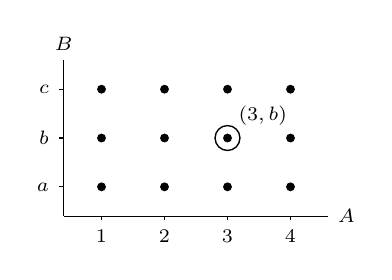
\begin{tikzpicture}[font=\scriptsize, x=0.8cm, y=0.62cm]
\draw[line width=0.4pt] (0.4,0.4) -- (4.6,0.4);
\draw[line width=0.4pt] (0.4,0.4) -- (0.4,3.6);
\foreach \i in {1,...,4} {\draw[line width=0.4pt] (\i,0.4) -- (\i,0.32); \node[below] at (\i,0.32) {$\i$};}
\foreach \j/\l in {1/a,2/b,3/c} {\draw[line width=0.4pt] (0.4,\j) -- (0.32,\j); \node[left] at (0.32,\j) {$\l$};}
\foreach \i in {1,...,4} \foreach \j in {1,2,3} {\fill (\i,\j) circle (1.6pt);}
\draw[line width=0.5pt] (3,2) circle (4.5pt);
\node[above right] at (3.02,2.05) {$(3,b)$};
\node[anchor=west] at (4.6,0.4) {$A$};
\node[anchor=south] at (0.4,3.6) {$B$};
\end{tikzpicture}}\hfill
\sdpanel{B}{\begin{tikzpicture}
\begin{axis}[sddiagram, width=5.2cm, height=3.9cm, xmin=-0.3, xmax=4.2, ymin=-0.3, ymax=2.9,
  xtick={1,3}, ytick={1,2}, xlabel={$x$}, ylabel={$y$}]
\fill[sdfill] (axis cs:1,1) rectangle (axis cs:3,2);
\draw[line width=0.5pt] (axis cs:1,1) rectangle (axis cs:3,2);
\draw[line width=1.4pt] (axis cs:1,0) -- (axis cs:3,0);
\draw[line width=1.4pt] (axis cs:0,1) -- (axis cs:0,2);
\draw[black!55, dashed, line width=0.4pt] (axis cs:1,0) -- (axis cs:1,1) (axis cs:3,0) -- (axis cs:3,1);
\draw[black!55, dashed, line width=0.4pt] (axis cs:0,1) -- (axis cs:1,1) (axis cs:0,2) -- (axis cs:1,2);
\node[font=\scriptsize] at (axis cs:2,1.5) {$[1,3]\times[1,2]$};
\end{axis}
\end{tikzpicture}}
\caption{Cartesian products. (A) The product of $A=\{1,2,3,4\}$ and $B=\{a,b,c\}$ as a grid of twelve pairs; the circled dot is the pair $(3,b)$. (B) The product $[1,3]\times[1,2]$ of two intervals (thick on the axes) is a rectangle in the plane $\mathbb R^2$.}
\label{fig:product}
\end{figure}

The product is not commutative: $A\times B$ and $B\times A$ are different sets unless $A=B$ or one of them is empty, because $(a,b)\ne(b,a)$ in general. If $A$ or $B$ is empty, then $A\times B=\emptyset$, since a pair needs a component from each set. The product interacts with the set operations as follows; the proofs are again translations into logic, and we prove one identity.

\begin{proposition}
\label{prop:product-laws}
For all sets $A$, $B$, $C$ and $D$:
\begin{enumerate}
\item $A\times(B\cup C)=(A\times B)\cup(A\times C)$ and $A\times(B\cap C)=(A\times B)\cap(A\times C)$;
\item $(A\times B)\cap(C\times D)=(A\cap C)\times(B\cap D)$;
\item $(A\times B)\cup(C\times D)\subseteq(A\cup C)\times(B\cup D)$, and the inclusion may be proper.
\end{enumerate}
\end{proposition}

\begin{proof}
We prove (ii). A pair $(x,y)$ lies in $(A\times B)\cap(C\times D)$ if and only if $x\in A$, $y\in B$, $x\in C$ and $y\in D$, and, after reordering the four conditions, this says that $x\in A\cap C$ and $y\in B\cap D$, that is, $(x,y)\in(A\cap C)\times(B\cap D)$. Every element of either side is a pair, so the two sets are equal. Part (i) is proved in the same way, and so is the inclusion in (iii). For the last claim of (iii), take $A=B=[0,1]$ and $C=D=[2,3]$: the pair $(0,2)$ lies in $(A\cup C)\times(B\cup D)$, but it lies neither in $A\times B$, since $2\notin B$, nor in $C\times D$, since $0\notin C$. Geometrically, the union of two squares on the diagonal is smaller than the large square that they span.
\end{proof}

\subsection{Tuples, Sequences, and Counting}

Ordered pairs generalise to any finite number of components. For $n\ge1$, an \term{$n$-tuple} $(a_1,\ldots,a_n)$ is determined by its components in order, so that $(a_1,\ldots,a_n)=(b_1,\ldots,b_n)$ if and only if $a_i=b_i$ for every $i$, and the product of sets $A_1,\ldots,A_n$ is
\[
A_1\times\cdots\times A_n\coloneqq\{(a_1,\ldots,a_n): a_i\in A_i\text{ for }i=1,\ldots,n\}.
\]
When all the factors are equal to $A$ we write $A^n$. Tuples of length three are called triples. The set $\mathbb R^n$ of $n$-tuples of real numbers is the setting of the linear algebra of Part~III, where its elements are called vectors. In computing, a record with fields of given types is an element of a product: a row of a table whose columns hold an integer, a real number and a name is an element of $\mathbb Z\times\mathbb R\times W$, where $W$ is the set of words, and a whole table with $m$ rows is an element of $(\mathbb Z\times\mathbb R\times W)^m$. Volume~VII builds data frames on this picture.

An \term{infinite sequence} $(a_0,a_1,a_2,\ldots)$, written $(a_n)_{n\in\mathbb N}$ as in \cref{def:sequence-limit}, is the infinite analogue of a tuple: it has a component $a_n$ for every $n\in\mathbb N$, and two sequences are equal when they agree in every component. \Cref{sec:functions} explains that a sequence is a particular kind of function, which settles what it is precisely.

For finite sets the size of a product is the product of the sizes, which explains the name.

\begin{proposition}
\label{prop:product-size}
If $A$ has $m$ elements and $B$ has $n$ elements, then $A\times B$ has $mn$ elements. Consequently, if $A$ has $m$ elements, then $A^k$ has $m^k$ elements for every $k\ge1$.
\end{proposition}

\begin{proof}
For each $a\in A$, the pairs with first component $a$ form the set $\{a\}\times B$, a row of the grid in \cref{fig:product}A. It has $n$ elements, one pair $(a,b)$ for each $b\in B$. The $m$ rows together make up $A\times B$, and two different rows have no pair in common, since pairs with different first components are different. Hence $A\times B$ has $n+n+\cdots+n=mn$ elements. The second statement follows by induction on $k$: identifying the $(k+1)$-tuple $(a_1,\ldots,a_k,a_{k+1})$ with the pair $\bigl((a_1,\ldots,a_k),a_{k+1}\bigr)$ shows that $A^{k+1}$ has as many elements as $A^k\times A$, namely $m^k\cdot m=m^{k+1}$.
\end{proof}

For instance, a binary word of $64$ bits is an element of $\{0,1\}^{64}$, and there are $2^{64}=18\,446\,744\,073\,709\,551\,616$ of them. This is the number of distinct values of a $64$-bit integer, and also the number of distinct bit patterns of a $64$-bit floating-point number; Volume~V explains why the floating-point numbers represented by these patterns are slightly fewer. The counting arguments used here informally, splitting a set into disjoint parts and adding their sizes, are justified in Chapter~4.

\section{Functions}
\label{sec:functions}

The idea of a function, a rule that turns an input into an output, is the notion that this series uses more than any other. Calculus studies functions of real numbers, linear algebra studies linear functions between vectors, and every routine in a numerical library computes a function. This section gives the definition and the basic operations on functions.

\subsection{Definition and Examples}

\begin{definition}[Function]
\label{def:function}
Let $A$ and $B$ be sets. A \term{function} $f$ from $A$ to $B$, written $f\colon A\to B$, assigns to each element $a\in A$ exactly one element $f(a)\in B$, the \term{value} of $f$ at $a$. The set $A$ is the \term{domain} of $f$ and $B$ its \term{codomain}. The \term{graph} of $f$ is the set
\[
\Gamma_f\coloneqq\{(a,f(a)): a\in A\}\subseteq A\times B .
\]
Two functions $f$ and $g$ are \term{equal} if they have the same domain $A$, the same codomain and $f(a)=g(a)$ for every $a\in A$.
\end{definition}

The words \term{map}, \term{mapping} and \term{transformation} are used as synonyms of ``function''. To define a function one must specify three things: the domain, the codomain and the rule. We write $a\mapsto f(a)$ to show the rule, as in ``the function $f\colon\mathbb R\to\mathbb R$, $x\mapsto x^2$''. The arrow $\mapsto$ goes from an element to an element, while $\to$ goes from a set to a set.

The phrase ``exactly one'' in \cref{def:function} contains two requirements: every element of the domain has a value (existence), and no element has two values (uniqueness). In terms of the graph, a subset $\Gamma\subseteq A\times B$ is the graph of a function from $A$ to $B$ if and only if
\[
\forall a\in A,\ \exists!\,b\in B,\ (a,b)\in\Gamma ,
\]
and the function is then determined by its graph. Axiomatic set theory takes this as the definition and identifies a function with its graph~\cite{enderton1977sets}. Since the graph alone does not record the codomain, authors who, like us, regard the codomain as part of the function define a function as the triple $(A,B,\Gamma)$ instead. For real functions the condition is the familiar vertical line test: every vertical line through a point of the domain meets the graph exactly once.

Here are some functions that occur throughout the series.
\begin{itemize}
\item Formulas: $f\colon\mathbb R\to\mathbb R$, $f(x)=x^2-3x+1$, and every polynomial in the same way.
\item The \term{identity function} $\operatorname{id}_A\colon A\to A$, $\operatorname{id}_A(a)=a$, and the \term{constant functions} $a\mapsto c$ for a fixed $c\in B$.
\item The \term{inclusion} $\iota\colon S\to A$, $\iota(s)=s$, of a subset $S\subseteq A$. It has the same rule as $\operatorname{id}_S$ but a different codomain, and so, by \cref{def:function}, it is a different function.
\item The \term{projections} $p_1\colon A\times B\to A$, $(a,b)\mapsto a$, and $p_2\colon A\times B\to B$, $(a,b)\mapsto b$. A function whose domain is a product, such as $(x,y)\mapsto x^2+y^2$ on $\mathbb R^2$, is a function of several variables; we write $f(x,y)$ for $f((x,y))$.
\item The \term{indicator function} $\mathbf 1_S\colon A\to\{0,1\}$ of a subset $S\subseteq A$, with $\mathbf 1_S(a)=1$ if $a\in S$ and $\mathbf 1_S(a)=0$ if $a\notin S$. It is also called the characteristic function of $S$, a name that we avoid because probability theory uses it for something else (Volume~III).
\item Sequences: a sequence $(a_n)_{n\in\mathbb N}$ of real numbers is a function $a\colon\mathbb N\to\mathbb R$, written with the argument as a subscript, $a_n$ instead of $a(n)$. Similarly, an $n$-tuple of elements of $B$ is a function $\{1,\ldots,n\}\to B$.
\item Arrays: an array of $n$ real numbers, indexed from $0$ as in most programming languages, is a function $\{0,1,\ldots,n-1\}\to\mathbb R$, and a table of $m$ rows and $n$ columns is a function $\{0,\ldots,m-1\}\times\{0,\ldots,n-1\}\to\mathbb R$. This point of view underlies Volume~VI.
\end{itemize}

It is equally important to recognise what is not a function. The rule ``assign to $x$ the number $y$ with $y^2=x$'' does not define a function from $\mathbb R$ to $\mathbb R$: for $x=-1$ there is no such $y$, so existence fails, and for $x=4$ there are two, $2$ and $-2$, so uniqueness fails. Both defects can be repaired by changing the sets: $x\mapsto\sqrt x$ is a function from $[0,\infty)$ to $\mathbb R$, by \cref{asm:numbers}\,(iv). Similarly, $x\mapsto1/x$ is a function on $\mathbb R\setminus\{0\}$ but not on $\mathbb R$. A function is not required to be given by a formula; ``$f(n)$ is the $n$th prime number'' and ``$f(x)=1$ if $x$ is rational and $0$ otherwise'' are perfectly good functions.

For sets $A$ and $B$, the set of all functions from $A$ to $B$ is written $B^A$. The notation is explained by the count: if $A$ has $m$ elements and $B$ has $n$, then a function is specified by choosing one of the $n$ values for each of the $m$ elements of $A$, and there are $n^m$ ways to do so (Chapter~4 makes this precise). For example, the set $\{0,1\}^{\mathbb N}$ is the set of all infinite sequences of zeros and ones. The indicator functions give a one-to-one correspondence between the subsets of $A$ and the functions $A\to\{0,1\}$: each subset $S$ yields $\mathbf 1_S$, and each function $g\colon A\to\{0,1\}$ is the indicator function of exactly one subset, namely $\{a\in A: g(a)=1\}$. This explains once more why a set of $n$ elements has $2^n$ subsets (\cref{prop:power-set-size}).

\subsection{Images and Preimages}

A function can be applied to a whole set of inputs at once, and it can be asked which inputs lead to a given set of outputs.

\begin{definition}[Image, preimage, range]
\label{def:image}
Let $f\colon A\to B$ be a function.
\begin{enumerate}
\item For $S\subseteq A$, the \term{image} of $S$ under $f$ is $f(S)\coloneqq\{f(s): s\in S\}\subseteq B$.
\item For $T\subseteq B$, the \term{preimage}, or inverse image, of $T$ under $f$ is $f^{-1}(T)\coloneqq\{a\in A: f(a)\in T\}\subseteq A$.
\end{enumerate}
The image $f(A)$ of the whole domain is the \term{range} of $f$.
\end{definition}

The image $f(S)$ is the set of outputs produced by inputs from $S$; the preimage $f^{-1}(T)$ is the set of inputs whose outputs land in $T$. The notation $f^{-1}(T)$ is used for every function, whether or not $f$ has an inverse function in the sense of \cref{sec:injections}. When it does, the two meanings of $f^{-1}$ agree, as we shall see. The range is a subset of the codomain, and it may be a proper subset: the function $x\mapsto x^2$ from $\mathbb R$ to $\mathbb R$ has codomain $\mathbb R$ and range $[0,\infty)$.

For $f\colon\mathbb R\to\mathbb R$, $f(x)=x^2$, we have
\begin{gather*}
f([1,2])=[1,4],\qquad f([-1,2])=[0,4],\\
f^{-1}([1,4])=[-2,-1]\cup[1,2],\qquad f^{-1}([-2,-1])=\emptyset .
\end{gather*}
The preimage of a set that the function never reaches is empty. \Cref{fig:image-preimage} shows images and preimages for a function between finite sets and for this function.

\begin{figure}
\tikzset{fdot/.style={circle, fill=black, inner sep=0pt, minimum size=3.2pt},
  farr/.style={-{Latex[length=1.4mm]}, line width=0.4pt, shorten >=1.5pt, shorten <=1.5pt}}
\sdpanel{A}{\begin{tikzpicture}[font=\scriptsize]
\fill[sdfill, rounded corners=4pt] (-0.36,1.85) rectangle (0.3,3.35);
\fill[sdfill, rounded corners=4pt] (2.2,2.7) rectangle (2.86,3.3);
\draw[line width=0.4pt] (0,1.8) ellipse (0.72 and 1.72);
\draw[line width=0.4pt] (2.5,1.8) ellipse (0.72 and 1.72);
\foreach \y/\l [count=\i] in {3.0/1,2.2/2,1.4/3,0.6/4} {\node[fdot] (a\i) at (0,\y) {}; \node[left=1pt] at (a\i) {$\l$};}
\foreach \y/\l [count=\i] in {3.0/a,2.2/b,1.4/c,0.6/d} {\node[fdot] (b\i) at (2.5,\y) {}; \node[right=1pt] at (b\i) {$\l$};}
\draw[farr] (a1) -- (b1); \draw[farr] (a2) -- (b1); \draw[farr] (a3) -- (b3); \draw[farr] (a4) -- (b3);
\node at (0,-0.2) {$A$}; \node at (2.5,-0.2) {$B$};
\node[anchor=east] at (-0.78,2.6) {$S$};
\node[anchor=west] at (3.26,3.0) {$f(S)$};
\end{tikzpicture}}\hfill
\sdpanel{B}{\begin{tikzpicture}
\begin{axis}[sddiagram, width=5.6cm, height=4.6cm, xmin=-2.6, xmax=2.6, ymin=-0.6, ymax=5.2,
  xtick={-2,-1,1,2}, ytick={1,4}, xlabel={$x$}, ylabel={$f(x)$}, clip=false,
  yticklabel style={fill=white, inner sep=1pt}]
\addplot[black, line width=0.6pt, domain=-2.25:2.25, samples=100] {x^2};
\draw[line width=1.6pt] (axis cs:0,1) -- (axis cs:0,4);
\draw[line width=1.6pt] (axis cs:-2,0) -- (axis cs:-1,0) (axis cs:1,0) -- (axis cs:2,0);
\draw[black!55, dashed, line width=0.4pt] (axis cs:-2,4) -- (axis cs:2,4) (axis cs:-1,1) -- (axis cs:1,1);
\draw[black!55, dashed, line width=0.4pt] (axis cs:-2,0) -- (axis cs:-2,4) (axis cs:2,0) -- (axis cs:2,4) (axis cs:-1,0) -- (axis cs:-1,1) (axis cs:1,0) -- (axis cs:1,1);
\node[font=\scriptsize, anchor=west] at (axis cs:0.12,2.6) {$T$};
\end{axis}
\end{tikzpicture}}
\caption{Images and preimages. (A) A function $f\colon A\to B$ drawn with arrows. The image of $S=\{1,2\}$ is $f(S)=\{a\}$ (shaded), the range is $f(A)=\{a,c\}$, and the preimage of $\{b,c\}$ is $f^{-1}(\{b,c\})=\{3,4\}$. (B) For $f(x)=x^2$ the preimage of $T=[1,4]$ (thick on the vertical axis) is $[-2,-1]\cup[1,2]$ (thick on the horizontal axis).}
\label{fig:image-preimage}
\end{figure}

Preimages are better behaved than images: they are compatible with all the set operations, while images are compatible only with unions.

\begin{proposition}
\label{prop:image-preimage}
Let $f\colon A\to B$ be a function, let $S,S_1,S_2\subseteq A$ and $T,T_1,T_2\subseteq B$, and let $(T_i)_{i\in I}$ be a family of subsets of $B$.
\begin{enumerate}
\item $f^{-1}(T_1\cup T_2)=f^{-1}(T_1)\cup f^{-1}(T_2)$ and $f^{-1}(T_1\cap T_2)=f^{-1}(T_1)\cap f^{-1}(T_2)$; more generally $f^{-1}\bigl(\bigcup_iT_i\bigr)=\bigcup_if^{-1}(T_i)$ and, for $I\ne\emptyset$, $f^{-1}\bigl(\bigcap_iT_i\bigr)=\bigcap_if^{-1}(T_i)$.
\item $f^{-1}(T_1\setminus T_2)=f^{-1}(T_1)\setminus f^{-1}(T_2)$; in particular $f^{-1}(B\setminus T)=A\setminus f^{-1}(T)$.
\item $f(S_1\cup S_2)=f(S_1)\cup f(S_2)$.
\item $f(S_1\cap S_2)\subseteq f(S_1)\cap f(S_2)$, and the inclusion may be proper.
\item $S\subseteq f^{-1}(f(S))$ and $f(f^{-1}(T))\subseteq T$, and both inclusions may be proper.
\end{enumerate}
\end{proposition}

\begin{proof}
(i) For $a\in A$,
\begin{align*}
a\in f^{-1}\Bigl(\bigcup_{i\in I}T_i\Bigr)&\iff f(a)\in\bigcup_{i\in I}T_i\iff\exists i\in I,\ f(a)\in T_i\\
&\iff\exists i\in I,\ a\in f^{-1}(T_i)\iff a\in\bigcup_{i\in I}f^{-1}(T_i),
\end{align*}
and the same chain with $\forall$ in place of $\exists$ proves the statement for intersections. The statements for two sets are the case $I=\{1,2\}$.

(ii) For $a\in A$: $a\in f^{-1}(T_1\setminus T_2)$ if and only if $f(a)\in T_1$ and $f(a)\notin T_2$, that is, $a\in f^{-1}(T_1)$ and $a\notin f^{-1}(T_2)$. The special case is $T_1=B$, using $f^{-1}(B)=A$.

(iii) Let $b\in f(S_1\cup S_2)$, say $b=f(s)$ with $s\in S_1\cup S_2$. If $s\in S_1$, then $b\in f(S_1)$; if $s\in S_2$, then $b\in f(S_2)$; in either case $b\in f(S_1)\cup f(S_2)$. Conversely, $S_1\subseteq S_1\cup S_2$ implies $f(S_1)\subseteq f(S_1\cup S_2)$, since every output produced from $S_1$ is produced from the larger set, and likewise for $S_2$.

(iv) If $b\in f(S_1\cap S_2)$, then $b=f(s)$ with $s$ in both $S_1$ and $S_2$, so $b\in f(S_1)$ and $b\in f(S_2)$. For an example of a proper inclusion, take $f(x)=x^2$ on $\mathbb R$, $S_1=\{-1\}$ and $S_2=\{1\}$. Then $S_1\cap S_2=\emptyset$ and $f(S_1\cap S_2)=\emptyset$, while $f(S_1)\cap f(S_2)=\{1\}$.

(v) If $s\in S$, then $f(s)\in f(S)$, so $s\in f^{-1}(f(S))$. If $b\in f(f^{-1}(T))$, then $b=f(a)$ for some $a$ with $f(a)\in T$, so $b\in T$. With $f(x)=x^2$ on $\mathbb R$, $S=\{1\}$ gives $f^{-1}(f(S))=\{-1,1\}\ne S$, and $T=[-1,1]$ gives $f(f^{-1}(T))=f([-1,1])=[0,1]\ne T$.
\end{proof}

The failure in (iv) comes from two different inputs with the same output: $-1$ and $1$ are separated by $S_1$ and $S_2$, but their common output $1$ is not. \Cref{sec:injections} shows that (iv) and the first half of (v) become equalities when this cannot happen. The good behaviour of preimages is the reason why many central definitions are made with them. In Volume~II, for instance, a function between metric spaces is shown to be continuous exactly when the preimage of every open set is open, and in Volume~III a random variable is defined as a function whose preimages of intervals are events.

\subsection{Restriction and Composition}

\begin{definition}[Restriction]
\label{def:restriction}
Let $f\colon A\to B$ and $S\subseteq A$. The \term{restriction} of $f$ to $S$ is the function $f|_S\colon S\to B$, $f|_S(s)=f(s)$.
\end{definition}

The restriction keeps the rule and the codomain and shrinks the domain. It is a different function from $f$ when $S\ne A$. For instance, $x\mapsto x^2$ on $\mathbb R$ and its restriction to $[0,\infty)$ have quite different properties, as the next section shows.

Functions can be applied one after another, the output of the first becoming the input of the second.

\begin{definition}[Composition]
\label{def:composition}
Let $f\colon A\to B$ and $g\colon B\to C$. The \term{composition} of $g$ with $f$ is the function
\[
g\circ f\colon A\to C,\qquad(g\circ f)(a)\coloneqq g(f(a)).
\]
\end{definition}

The composition $g\circ f$, read ``$g$ after $f$'', applies $f$ first, although $f$ is written second; the order follows the notation $g(f(a))$, in which the function nearest the argument acts first. The composition is defined only when the codomain of $f$ is the domain of $g$. Many authors require only that the range of $f$ be contained in the domain of $g$; with \cref{def:composition} such a composition is formed by first changing the codomain of $f$.

Composition is not commutative. For $f(x)=x+1$ and $g(x)=x^2$ on $\mathbb R$,
\[
(g\circ f)(x)=(x+1)^2,\qquad(f\circ g)(x)=x^2+1,
\]
and these functions differ, for example at $x=1$, where they take the values $4$ and $2$. Composition is, however, associative, and the identity functions act as neutral elements.

\begin{proposition}
\label{prop:composition}
Let $f\colon A\to B$, $g\colon B\to C$ and $h\colon C\to D$. Then
\[
h\circ(g\circ f)=(h\circ g)\circ f
\qquad\text{and}\qquad
f\circ\operatorname{id}_A=f=\operatorname{id}_B\circ f .
\]
\end{proposition}

\begin{proof}
Both sides of the first identity are functions from $A$ to $D$. For every $a\in A$,
\[
\bigl(h\circ(g\circ f)\bigr)(a)=h\bigl((g\circ f)(a)\bigr)=h\bigl(g(f(a))\bigr)
=(h\circ g)\bigl(f(a)\bigr)=\bigl((h\circ g)\circ f\bigr)(a),
\]
so the two functions are equal by \cref{def:function}. Similarly $(f\circ\operatorname{id}_A)(a)=f(a)=(\operatorname{id}_B\circ f)(a)$ for every $a\in A$.
\end{proof}

Because of associativity we write $h\circ g\circ f$ without parentheses. A long computation is a composition of many simple steps, and associativity says that the steps may be grouped in any way without changing the result. (In floating-point arithmetic, it is the grouping of \emph{additions}, not of function compositions, that matters, a distinction drawn in Volume~V.) Images and preimages behave well under composition: $(g\circ f)(S)=g(f(S))$ and $(g\circ f)^{-1}(U')=f^{-1}(g^{-1}(U'))$ for $S\subseteq A$ and $U'\subseteq C$, as one checks directly from the definitions.

\section{Injections, Surjections, and Bijections}
\label{sec:injections}

The function $x\mapsto x^2$ on $\mathbb R$ cannot be undone: from the output $4$ one cannot tell whether the input was $2$ or $-2$, and the output $-1$ never occurs. These are the two ways in which a function can fail to be reversible, and they lead to the central definitions of this section~\cite{velleman2019,halmos1960naive}.

\subsection{Definitions and Examples}

\begin{definition}[Injective, surjective, bijective]
\label{def:injective}
A function $f\colon A\to B$ is
\begin{enumerate}
\item \term{injective}, or one-to-one, if different inputs have different outputs: for all $a,a'\in A$, $f(a)=f(a')\Rightarrow a=a'$;
\item \term{surjective}, or onto, if every element of the codomain is an output: for every $b\in B$ there is $a\in A$ with $f(a)=b$, that is, $f(A)=B$;
\item \term{bijective} if it is both injective and surjective.
\end{enumerate}
An injective function is called an \term{injection}, a surjective one a \term{surjection} and a bijective one a \term{bijection}, or a one-to-one correspondence.
\end{definition}

In terms of equations, $f$ is injective if every equation $f(x)=b$ with $b\in B$ has at most one solution $x\in A$, surjective if every such equation has at least one solution, and bijective if every such equation has exactly one solution. In the arrow pictures of \cref{fig:kinds}, injectivity means that no two arrows arrive at the same point, and surjectivity means that every point of the codomain receives an arrow. For a real function, injectivity means that every horizontal line meets the graph at most once, and surjectivity that every horizontal line at a height in the codomain meets it at least once.

\begin{figure}
\tikzset{fdot/.style={circle, fill=black, inner sep=0pt, minimum size=3.2pt},
  farr/.style={-{Latex[length=1.4mm]}, line width=0.4pt, shorten >=1.5pt, shorten <=1.5pt}}
\newcommand\kindpanel[4]{%
\begin{tikzpicture}[font=\scriptsize]
\draw[line width=0.4pt] (0,1.25) ellipse (0.42 and 1.3);
\draw[line width=0.4pt] (1.75,1.25) ellipse (0.42 and 1.3);
\foreach \y [count=\i] in {#1} {\node[fdot] (a\i) at (0,\y) {};}
\foreach \y [count=\i] in {#2} {\node[fdot] (b\i) at (1.75,\y) {};}
\foreach \s/\t in {#3} {\draw[farr] (a\s) -- (b\t);}
\node at (0,-0.3) {$A$}; \node at (1.75,-0.3) {$B$};
\node[font=\scriptsize, align=center] at (0.875,-0.78) {#4};
\end{tikzpicture}}
\sdpanel{A}{\kindpanel{2,1.25,0.5}{2,1.25,0.5}{1/1,2/1,3/2}{neither}}\hfill
\sdpanel{B}{\kindpanel{1.9,1.25,0.6}{2.1,1.5,0.95,0.4}{1/1,2/2,3/4}{injective}}\hfill
\sdpanel{C}{\kindpanel{2.1,1.5,0.95,0.4}{1.9,1.25,0.6}{1/1,2/2,3/3,4/3}{surjective}}\hfill
\sdpanel{D}{\kindpanel{2,1.25,0.5}{2,1.25,0.5}{1/2,2/3,3/1}{bijective}}
\caption{The kinds of functions. (A) Two arrows meet and one point of $B$ is missed: neither injective nor surjective. (B) No two arrows meet, but a point of $B$ is missed: injective, not surjective. (C) Every point of $B$ is hit, but two arrows meet: surjective, not injective. (D) Every point of $B$ is hit exactly once: bijective.}
\label{fig:kinds}
\end{figure}

The square function shows that the three properties depend on the domain and the codomain as much as on the rule. Let $Q=[0,\infty)$.
\begin{itemize}
\item $x\mapsto x^2$ from $\mathbb R$ to $\mathbb R$ is neither injective ($(-1)^2=1^2$) nor surjective ($-1$ is not a square).
\item $x\mapsto x^2$ from $Q$ to $\mathbb R$ is injective but not surjective. If $x,y\ge0$ and $x^2=y^2$, then $0=x^2-y^2=(x-y)(x+y)$, so $x=y$ or $x+y=0$, and the latter forces $x=y=0$.
\item $x\mapsto x^2$ from $\mathbb R$ to $Q$ is surjective but not injective: every $y\ge0$ equals $(\sqrt y)^2$ by \cref{asm:numbers}\,(iv).
\item $x\mapsto x^2$ from $Q$ to $Q$ is bijective, by the two previous arguments.
\end{itemize}

More examples:
\begin{itemize}
\item For real numbers $a\ne0$ and $b$, the function $x\mapsto ax+b$ from $\mathbb R$ to $\mathbb R$ is bijective, because the equation $ax+b=c$ has exactly one solution for every $c$ (\cref{prop:linear-equation}).
\item On the integers, $n\mapsto n+1$ is a bijection from $\mathbb Z$ to $\mathbb Z$, and $n\mapsto2n$ is an injection that is not surjective, since its range $2\mathbb Z$ misses the odd integers.
\item On the natural numbers, $n\mapsto n+1$ is an injection that is not surjective, since $0$ is not of the form $n+1$ with $n\in\mathbb N$. The halving function $h\colon\mathbb N\to\mathbb N$, $h(n)=(n-n\bmod2)/2$, which discards the last binary digit, is surjective, since $h(2m)=m$, but not injective, since $h(2m)=h(2m+1)$.
\item The projection $p_1\colon A\times B\to A$ is surjective when $B\ne\emptyset$ and injective when $B$ has at most one element.
\item The inclusion of a subset is always injective, and an identity function is always bijective.
\end{itemize}

To prove that a function is injective, the definition suggests the standard pattern: assume $f(a)=f(a')$ and deduce $a=a'$, as in the argument for $x^2$ on $Q$ above. To prove that it is surjective, take an arbitrary $b$ in the codomain and exhibit an $a$ with $f(a)=b$, usually by solving the equation $f(a)=b$. A function that is not injective is refuted by two different inputs with the same output, and a function that is not surjective by one element of the codomain that is never an output.

An injective function preserves the distinctions that \cref{prop:image-preimage} lost. If $f$ is injective, then $f(S_1\cap S_2)=f(S_1)\cap f(S_2)$ and $f^{-1}(f(S))=S$ for all subsets $S,S_1,S_2$ of the domain. If $f$ is surjective, then $f(f^{-1}(T))=T$ for every subset $T$ of the codomain. In view of \cref{prop:image-preimage}, only one inclusion has to be shown in each case. An element $b\in f(S_1)\cap f(S_2)$ is of the form $b=f(s_1)=f(s_2)$ with $s_1\in S_1$ and $s_2\in S_2$, and injectivity gives $s_1=s_2\in S_1\cap S_2$, so $b\in f(S_1\cap S_2)$. An element $a\in f^{-1}(f(S))$ satisfies $f(a)=f(s)$ for some $s\in S$, and injectivity gives $a=s\in S$. Finally, if $f$ is surjective and $b\in T$, then $b=f(a)$ for some $a$, which lies in $f^{-1}(T)$, so $b\in f(f^{-1}(T))$.

\subsection{Composition}

The three properties are preserved by composition, and partly inherited backwards from a composition.

\begin{proposition}
\label{prop:composition-injective}
Let $f\colon A\to B$ and $g\colon B\to C$.
\begin{enumerate}
\item If $f$ and $g$ are injective, so is $g\circ f$.
\item If $f$ and $g$ are surjective, so is $g\circ f$.
\item If $f$ and $g$ are bijective, so is $g\circ f$.
\item If $g\circ f$ is injective, then $f$ is injective.
\item If $g\circ f$ is surjective, then $g$ is surjective.
\end{enumerate}
\end{proposition}

\begin{proof}
(i) Suppose $g(f(a))=g(f(a'))$. Since $g$ is injective, $f(a)=f(a')$, and since $f$ is injective, $a=a'$.

(ii) Let $c\in C$. Since $g$ is surjective, $c=g(b)$ for some $b\in B$, and since $f$ is surjective, $b=f(a)$ for some $a\in A$. Then $c=g(f(a))$.

(iii) This follows from (i) and (ii).

(iv) Suppose $f(a)=f(a')$. Applying $g$ gives $g(f(a))=g(f(a'))$, and since $g\circ f$ is injective, $a=a'$.

(v) Let $c\in C$. Since $g\circ f$ is surjective, $c=g(f(a))$ for some $a\in A$, so $c$ is the value of $g$ at the element $f(a)$ of $B$.
\end{proof}

Parts (iv) and (v) cannot be reversed. Let $A=\{0\}$, $B=\{0,1\}$ and $C=\{0\}$, let $f(0)=0$, and let $g$ send both elements of $B$ to $0$. Then $g\circ f\colon\{0\}\to\{0\}$ is bijective, but $g$ is not injective and $f$ is not surjective.

\subsection{Inverse Functions}

\begin{definition}[Inverse function]
\label{def:inverse}
Let $f\colon A\to B$. A function $g\colon B\to A$ is an \term{inverse} of $f$ if
\[
g\circ f=\operatorname{id}_A\qquad\text{and}\qquad f\circ g=\operatorname{id}_B ,
\]
that is, if $g(f(a))=a$ for every $a\in A$ and $f(g(b))=b$ for every $b\in B$. A function that has an inverse is \term{invertible}.
\end{definition}

An inverse undoes $f$ from either side. The main theorem of this section identifies the invertible functions.

\begin{theorem}[Inverse functions]
\label{thm:inverse}
A function $f\colon A\to B$ has an inverse if and only if it is bijective. The inverse is then unique; it is denoted $f^{-1}$, and $f^{-1}(b)$ is the unique $a\in A$ with $f(a)=b$. Moreover, $f^{-1}$ is bijective and $(f^{-1})^{-1}=f$.
\end{theorem}

\begin{proof}
($\Rightarrow$) Suppose $g$ is an inverse of $f$. Then $g\circ f=\operatorname{id}_A$ is injective, so $f$ is injective by \cref{prop:composition-injective}\,(iv), and $f\circ g=\operatorname{id}_B$ is surjective, so $f$ is surjective by \cref{prop:composition-injective}\,(v).

($\Leftarrow$) Suppose $f$ is bijective. For each $b\in B$ the equation $f(a)=b$ has exactly one solution $a\in A$: at least one because $f$ is surjective and at most one because it is injective. Define $g(b)$ to be this solution. Then $f(g(b))=b$ for every $b\in B$, by the definition of $g$. For $a\in A$, the element $g(f(a))$ is the unique solution of the equation $f(x)=f(a)$, and $x=a$ is a solution, so $g(f(a))=a$. Hence $g$ is an inverse of $f$.

\emph{Uniqueness.} Let $g$ and $h$ both be inverses of $f$. By \cref{prop:composition},
\[
g=g\circ\operatorname{id}_B=g\circ(f\circ h)=(g\circ f)\circ h=\operatorname{id}_A\circ h=h .
\]
The description of $f^{-1}(b)$ is the construction in the proof of ($\Leftarrow$). Finally, the two equations of \cref{def:inverse} are symmetric in $f$ and $g$, so $f$ is an inverse of $f^{-1}$; hence $f^{-1}$ is bijective by ($\Rightarrow$), and $(f^{-1})^{-1}=f$ by uniqueness.
\end{proof}

For a bijection $f$ the notation $f^{-1}$ now has two meanings, the inverse function and the preimage of \cref{def:image}. They are consistent: for every $T\subseteq B$, the preimage of $T$ under $f$ equals the image of $T$ under the inverse function, and in particular the preimage of $\{b\}$ is $\{f^{-1}(b)\}$.

The inverse of the bijection $x\mapsto x^2$ on $[0,\infty)$ is the square root $y\mapsto\sqrt y$ on $[0,\infty)$; the inverse of $x\mapsto ax+b$ on $\mathbb R$, with $a\ne0$, is $y\mapsto(y-b)/a$. The graph of an inverse function consists of the pairs of the graph of $f$ with their components exchanged, $\Gamma_{f^{-1}}=\{(b,a): (a,b)\in\Gamma_f\}$. For real functions this exchange is the reflection in the diagonal line $y=x$, as \cref{fig:inverse-graph} shows.

\begin{figure}
\sdfloat{%
\begin{tikzpicture}
\begin{axis}[sdplot, width=5.4cm, height=5.4cm, xmin=0, xmax=2.7, ymin=0, ymax=2.7,
  xtick={0,1,2}, ytick={0,1,2}, xlabel={$x$}, ylabel={$y$}, clip=false]
\addplot[black!45, dashed, line width=0.5pt, domain=0:2.6] {x};
\addplot[black, line width=0.7pt, domain=0:1.62, samples=80] {x^2};
\addplot[black, densely dotted, line width=0.8pt, domain=0:2.62, samples=200] {sqrt(x)};
\fill (axis cs:1.4,1.96) circle (1.4pt);
\fill (axis cs:1.96,1.4) circle (1.4pt);
\draw[black!55, line width=0.4pt] (axis cs:1.4,1.96) -- (axis cs:1.96,1.4);
\node[font=\scriptsize, anchor=east] at (axis cs:1.36,2.02) {$(a,b)$};
\node[font=\scriptsize, anchor=north west] at (axis cs:1.98,1.36) {$(b,a)$};
\node[font=\scriptsize, anchor=east] at (axis cs:1.52,2.62) {$y=x^2$};
\node[font=\scriptsize, anchor=west] at (axis cs:2.64,1.62) {$y=\sqrt x$};
\node[font=\scriptsize, anchor=west] at (axis cs:2.62,2.62) {$y=x$};
\end{axis}
\end{tikzpicture}}{A function and its inverse. The graph of $f(x)=x^2$ on $[0,\infty)$ (solid) and the graph of its inverse $f^{-1}(y)=\sqrt y$ (dotted) are mirror images in the diagonal $y=x$ (dashed): the point $(a,b)$ of one graph corresponds to the point $(b,a)$ of the other.\label{fig:inverse-graph}}
\end{figure}

\begin{proposition}
\label{prop:inverse-composition}
If $f\colon A\to B$ and $g\colon B\to C$ are bijective, then $(g\circ f)^{-1}=f^{-1}\circ g^{-1}$.
\end{proposition}

\begin{proof}
By \cref{prop:composition-injective}\,(iii), $g\circ f$ is bijective. Using associativity,
\[
(f^{-1}\circ g^{-1})\circ(g\circ f)=f^{-1}\circ(g^{-1}\circ g)\circ f=f^{-1}\circ\operatorname{id}_B\circ f=f^{-1}\circ f=\operatorname{id}_A,
\]
and in the same way $(g\circ f)\circ(f^{-1}\circ g^{-1})=\operatorname{id}_C$. So $f^{-1}\circ g^{-1}$ is an inverse of $g\circ f$, and by the uniqueness in \cref{thm:inverse} it is the inverse.
\end{proof}

The order is reversed for the same reason that one takes off one's shoes before one's socks: what was done last must be undone first.

A bijection from a set to itself is called a \term{permutation} of the set. The permutations of $\{0,1,\ldots,n-1\}$ describe the rearrangements of an array of length $n$: sorting an array, for instance, amounts to finding a permutation $\sigma$ such that the entry at position $\sigma(0)$ is the smallest, the entry at position $\sigma(1)$ the next, and so on. If $\sigma$ is the permutation of $\{0,1,2,3\}$ with $\sigma(0)=2$, $\sigma(1)=0$, $\sigma(2)=3$ and $\sigma(3)=1$, then its inverse is obtained by reading the assignments backwards: $\sigma^{-1}(2)=0$, $\sigma^{-1}(0)=1$, $\sigma^{-1}(3)=2$ and $\sigma^{-1}(1)=3$. Volume~VI uses permutations of this kind throughout, and Chapter~4 counts them.

\subsection{One-Sided Inverses}

A function that is only injective, or only surjective, can still be undone from one side.

\begin{proposition}
\label{prop:one-sided}
Let $f\colon A\to B$ be a function with $A\ne\emptyset$.
\begin{enumerate}
\item $f$ is injective if and only if it has a \term{left inverse}, a function $g\colon B\to A$ with $g\circ f=\operatorname{id}_A$.
\item $f$ is surjective if and only if it has a \term{right inverse}, a function $h\colon B\to A$ with $f\circ h=\operatorname{id}_B$.
\end{enumerate}
\end{proposition}

\begin{proof}
In both parts the implication from the inverse to the property is \cref{prop:composition-injective}\,(iv) and (v), since identity functions are bijective.

(i) Let $f$ be injective, and fix an element $a_0\in A$, which exists because $A\ne\emptyset$. For $b\in f(A)$ there is exactly one $a\in A$ with $f(a)=b$, by injectivity; let $g(b)$ be this $a$. For $b\in B\setminus f(A)$ let $g(b)\coloneqq a_0$. Then $g\colon B\to A$, and $g(f(a))=a$ for every $a\in A$, since $a$ is the unique element with value $f(a)$.

(ii) Let $f$ be surjective. For each $b\in B$ the preimage $f^{-1}(\{b\})$ is nonempty. Choose one of its elements and call it $h(b)$. Then $f(h(b))=b$ for every $b\in B$.
\end{proof}

The proof of (ii) makes a choice for every element of $B$ simultaneously, and when $B$ is infinite this is an application of the axiom of choice described in the note in \cref{sec:sets}. Conversely, the statement ``every surjection has a right inverse'' implies the axiom of choice, so the two are equivalent~\cite{bell2021choice}: for a family $(A_i)_{i\in I}$ of nonempty sets, the map $(i,a)\mapsto i$ from the set of pairs $(i,a)$ with $i\in I$ and $a\in A_i$ onto $I$ is surjective, and a right inverse of it assigns to each $i$ a pair $(i,a)$ with $a\in A_i$, that is, it selects an element of each $A_i$. In concrete cases no axiom is needed, because a rule for the choice is available: if $A\subseteq\mathbb N$, for instance, $h(b)$ can be taken to be the least element of $f^{-1}(\{b\})$, which exists by the well-ordering principle (\cref{thm:well-ordering}). For the surjective halving function $n\mapsto(n-n\bmod2)/2$ of the examples above, the functions $m\mapsto2m$ and $m\mapsto2m+1$ are two different right inverses, and neither is a left inverse. A one-sided inverse is in general not unique, in contrast to the two-sided inverse of \cref{thm:inverse}.

The square root on a computer illustrates the difference. The function $x\mapsto x^2$ from $\mathbb R$ onto $[0,\infty)$ is surjective, and the square root is the right inverse that picks the nonnegative preimage: $(\sqrt y)^2=y$ for every $y\ge0$, but $\sqrt{x^2}=|x|$, which differs from $x$ when $x<0$. Choosing a particular right inverse of a surjective function is how inverse trigonometric functions, logarithms of complex numbers and many other ``principal values'' are defined (Chapter~9 and Volume~II).

\section{Relations}
\label{sec:relations}

Mathematics is full of statements that relate two objects: $x<y$, $a\mid b$, $A\subseteq B$, ``$x$ and $y$ leave the same remainder''. Each of them is a predicate in two variables, and the pairs for which it is true form a set. This set is the relation~\cite{enderton1977sets}.

\subsection{Definition and Examples}

\begin{definition}[Relation]
\label{def:relation}
A \term{relation} from a set $A$ to a set $B$ is a subset $R\subseteq A\times B$. We write $a\mathrel{R}b$ for $(a,b)\in R$ and say that $a$ is related to $b$. A relation from $A$ to $A$ is a relation \term{on} $A$.
\end{definition}

The definition identifies a relation with its truth set, in the sense of \cref{def:predicate}. For example, the relation $<$ on $\mathbb R$ is the set $\{(x,y)\in\mathbb R^2: x<y\}$, the open half-plane above the diagonal, and $x<y$ is the same statement as $(x,y)\in{<}$. Some further relations that we use repeatedly:
\begin{itemize}
\item equality $=$ on any set $A$, which is the diagonal $\{(a,a): a\in A\}$ of $A\times A$;
\item the orders $\le$ and $<$ on $\mathbb N$, $\mathbb Z$, $\mathbb Q$ and $\mathbb R$;
\item divisibility $\mid$ on $\mathbb Z$ (\cref{def:even-odd});
\item inclusion $\subseteq$ on the power set $\mathcal P(X)$ of a set $X$;
\item \term{congruence modulo} $n$, for a fixed integer $n\ge1$: integers $a$ and $b$ are congruent modulo $n$, written $a\equiv b\pmod n$, if $n\mid a-b$. Thus $17\equiv2\pmod5$ and $-1\equiv3\pmod4$. Chapter~3 studies this relation in detail;
\item a relation from a set of people to a set of cities, ``$p$ has lived in $c$'', and in general any table with two columns, each row of which records one related pair.
\end{itemize}

A function $f\colon A\to B$ is a particular relation from $A$ to $B$, namely its graph $\Gamma_f$, in which each element of $A$ is related to exactly one element of $B$. A general relation may relate an element to none, one or many elements. Two operations on relations generalise operations on functions. The \term{inverse} of a relation $R$ from $A$ to $B$ is the relation $R^{-1}\coloneqq\{(b,a): (a,b)\in R\}$ from $B$ to $A$; for instance, the inverse of $<$ is $>$. Unlike the inverse function, the inverse relation always exists. If $R$ is a relation from $A$ to $B$ and $S$ a relation from $B$ to $C$, their \term{composition} is the relation from $A$ to $C$
\[
S\circ R\coloneqq\{(a,c)\in A\times C:\exists b\in B,\ a\mathrel{R}b\wedge b\mathrel{S}c\}.
\]
When $R$ and $S$ are graphs of functions $f$ and $g$, the composition $S\circ R$ is the graph of $g\circ f$, which explains the order of the letters. If ``$p$ is a parent of $q$'' is the relation $R$ on a set of people, then $R\circ R$ is ``$p$ is a grandparent of $q$''.

\subsection{Properties of Relations}

Four properties of a relation on a single set occur so often that they have names.

\begin{definition}[Reflexive, symmetric, antisymmetric, transitive]
\label{def:relation-properties}
A relation $R$ on a set $A$ is
\begin{enumerate}
\item \term{reflexive} if $a\mathrel{R}a$ for every $a\in A$;
\item \term{symmetric} if $a\mathrel{R}b$ implies $b\mathrel{R}a$, for all $a,b\in A$;
\item \term{antisymmetric} if $a\mathrel{R}b$ and $b\mathrel{R}a$ together imply $a=b$, for all $a,b\in A$;
\item \term{transitive} if $a\mathrel{R}b$ and $b\mathrel{R}c$ together imply $a\mathrel{R}c$, for all $a,b,c\in A$.
\end{enumerate}
\end{definition}

\Cref{tab:relation-properties} records these properties for a number of relations. Each entry is a small proposition. A ``yes'' must be proved for all elements, while a ``no'' needs only one counterexample, in accordance with \cref{thm:quantifier-negation}.

\begin{table}
\sdfloat{%
\begin{sdtable}{colspec={llcccc}, row{1}={font=\small\bfseries}}
\toprule
Relation & Set & Refl. & Symm. & Antisymm. & Trans. \\
\midrule
$a=b$ & any & yes & yes & yes & yes \\
$x\le y$ & $\mathbb R$ & yes & no & yes & yes \\
$x<y$ & $\mathbb R$ & no & no & yes & yes \\
$x\ne y$ & $\mathbb R$ & no & yes & no & no \\
$a\mid b$ & $\mathbb N$ & yes & no & yes & yes \\
$a\mid b$ & $\mathbb Z$ & yes & no & no & yes \\
$S\subseteq T$ & $\mathcal P(X)$, $X\ne\emptyset$ & yes & no & yes & yes \\
$a\equiv b\pmod n$ & $\mathbb Z$ & yes & yes & no & yes \\
$x^2=y^2$ & $\mathbb R$ & yes & yes & no & yes \\
$|x-y|<1$ & $\mathbb R$ & yes & yes & no & no \\
empty relation & $A\ne\emptyset$ & no & yes & yes & yes \\
\bottomrule
\end{sdtable}}{Properties of some relations. For congruence the modulus is an integer $n\ge1$. A ``no'' means that the property fails for at least one choice of elements.\label{tab:relation-properties}}
\end{table}

Let us verify a few entries. For $x\ne y$ on $\mathbb R$, transitivity fails because $1\ne2$ and $2\ne1$, but $1\ne1$ is false. For $|x-y|<1$, transitivity fails because $0$ is related to $0.6$ and $0.6$ to $1.2$, but $0$ is not related to $1.2$. Divisibility on $\mathbb N$ is antisymmetric: if $a\mid b$ and $b\mid a$ with $a,b\in\mathbb N$, then either $b=0$, in which case $b\mid a$ forces $a=0$; or $b\ne0$, in which case $a\ne0$ too and \cref{prop:divisibility}\,(iv) gives $a\le b$ and $b\le a$, so $a=b$. On $\mathbb Z$ antisymmetry fails, since $2\mid-2$ and $-2\mid2$. Transitivity of divisibility is \cref{prop:divisibility}\,(ii). For congruence modulo $n$: $n\mid a-a=0$ gives reflexivity; if $n\mid a-b$ then $n\mid b-a=-(a-b)$, which gives symmetry; and if $n\mid a-b$ and $n\mid b-c$, then $n\mid(a-b)+(b-c)=a-c$ by \cref{prop:divisibility}\,(iii), which gives transitivity. The empty relation is symmetric, antisymmetric and transitive vacuously, because no pair satisfies their hypotheses.

Antisymmetry is not the negation of symmetry. Equality is both symmetric and antisymmetric, and $|x-y|<1$ is neither of the two. A relation that is symmetric and antisymmetric can relate an element only to itself, because $a\mathrel{R}b$ then gives $b\mathrel{R}a$ and hence $a=b$.

\subsection{Pictures and Matrices}

A relation on a finite set $A$ can be drawn as a \term{directed graph}: the elements of $A$ are drawn as points, and an arrow is drawn from $a$ to $b$ whenever $a\mathrel{R}b$, a loop when $a=b$. It can also be written as a table of zeros and ones. If $A=\{a_1,\ldots,a_n\}$, the \term{matrix} of $R$ is the square array $M$ with $n$ rows and $n$ columns whose entry in row $i$ and column $j$ is
\[
M_{ij}=\begin{cases}1&\text{if }a_i\mathrel{R}a_j,\\0&\text{otherwise.}\end{cases}
\]
\Cref{fig:relation} shows both pictures for divisibility on $\{1,2,3,4,6\}$.

\begin{figure}
\tikzset{rv/.style={circle, draw, line width=0.4pt, minimum size=0.5cm, inner sep=0pt, font=\scriptsize},
  rarr/.style={-{Latex[length=1.4mm]}, line width=0.4pt},
  rloop/.style={-{Latex[length=1.2mm]}, line width=0.4pt, looseness=6}}
\sdpanel{A}{\begin{tikzpicture}
\node[rv] (n1) at (0,0) {$1$};
\node[rv] (n2) at (-1.1,1.2) {$2$};
\node[rv] (n3) at (1.3,1.2) {$3$};
\node[rv] (n4) at (-1.1,2.6) {$4$};
\node[rv] (n6) at (0.9,2.6) {$6$};
\draw[rarr] (n1) -- (n2); \draw[rarr] (n1) -- (n3); \draw[rarr] (n1) -- (n4); \draw[rarr] (n1) -- (n6);
\draw[rarr] (n2) -- (n4); \draw[rarr] (n2) -- (n6); \draw[rarr] (n3) -- (n6);
\draw[rloop] (n1) to[out=-60, in=-120] (n1);
\draw[rloop] (n2) to[out=150, in=210] (n2);
\draw[rloop] (n3) to[out=-30, in=30] (n3);
\draw[rloop] (n4) to[out=60, in=120] (n4);
\draw[rloop] (n6) to[out=30, in=90] (n6);
\end{tikzpicture}}\hfill
\sdpanel{B}{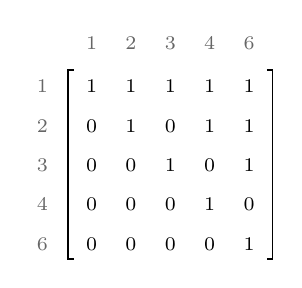
\begin{tikzpicture}[font=\scriptsize, x=0.5cm, y=0.5cm]
\foreach \l [count=\j] in {1,2,3,4,6} {\node[black!60, anchor=base] at (\j,-0.08) {$\l$}; \node[black!60, anchor=base] at (-0.25,-\j-0.18) {$\l$};}
\foreach \row [count=\i] in {{1,1,1,1,1},{0,1,0,1,1},{0,0,1,0,1},{0,0,0,1,0},{0,0,0,0,1}} {
  \foreach \e [count=\j] in \row {\node[anchor=base] at (\j,-\i-0.18) {$\e$};}}
\draw[line width=0.5pt] (0.55,-0.6) -- (0.4,-0.6) -- (0.4,-5.4) -- (0.55,-5.4);
\draw[line width=0.5pt] (5.45,-0.6) -- (5.6,-0.6) -- (5.6,-5.4) -- (5.45,-5.4);
\end{tikzpicture}}
\caption{Two pictures of the relation $a\mid b$ on $\{1,2,3,4,6\}$. (A) The directed graph: an arrow from $a$ to $b$ means that $a$ divides $b$; every element has a loop because the relation is reflexive. (B) The matrix: the entry in row $a$ and column $b$ is $1$ if $a\mid b$.}
\label{fig:relation}
\end{figure}

The properties of \cref{def:relation-properties} can be read off both pictures. A relation is reflexive when every point has a loop, or every diagonal entry of the matrix is $1$. It is symmetric when every arrow is matched by an arrow in the opposite direction, or the matrix is unchanged by reflecting it in its diagonal ($M_{ij}=M_{ji}$ for all $i$ and $j$; in the language of Chapter~13, $M$ equals its transpose). It is antisymmetric when no two different points are joined by arrows in both directions, or $M_{ij}$ and $M_{ji}$ are never both $1$ for $i\ne j$. Transitivity is a condition on paths of two arrows: whenever there are arrows from $a$ to $b$ and from $b$ to $c$, there must be an arrow from $a$ to $c$. In \cref{fig:relation}A, the path $1\to2\to4$ is accompanied by the arrow $1\to4$, and so on for every such path.

The matrix makes transitivity mechanically checkable. The condition is a universal statement over three indices,
\[
\forall i,\ \forall j,\ \forall k,\ \bigl(M_{ij}=1\wedge M_{jk}=1\Rightarrow M_{ik}=1\bigr),
\]
and, as in \cref{sec:quantifiers}, a universal statement over a finite domain is a loop. \Cref{alg:transitive} nests three loops, one for each quantifier, and returns false as soon as it finds a counterexample. It examines at most $n^3$ triples of indices, and its correctness is a direct reading of the quantified condition: it returns true exactly when no triple violates the implication.

\begin{algorithm}
\begin{algorithmic}[1]
\Require the matrix $M$ of a relation on a set of $n$ elements, $M_{ij}\in\{0,1\}$
\Ensure true if the relation is transitive, false otherwise
\Name{IsTransitive}{M}
\For{$i\gets1$ \textbf{to} $n$}
  \For{$j\gets1$ \textbf{to} $n$}
    \If{$M_{ij}=1$} \Comment{only pairs $a_i\mathrel{R}a_j$ can start a path}
      \For{$k\gets1$ \textbf{to} $n$}
        \If{$M_{jk}=1$ \textbf{and} $M_{ik}=0$} \Comment{a counterexample}
          \State \Return false
        \EndIf
      \EndFor
    \EndIf
  \EndFor
\EndFor
\State \Return true
\end{algorithmic}
\caption{Testing a relation for transitivity. The three loops correspond to the three universal quantifiers in the definition.}
\label{alg:transitive}
\end{algorithm}

\subsection{Transitive Closure}

A relation that is not transitive can be made transitive by adding pairs. If $R$ records the direct flights between cities, then ``one can fly from $a$ to $b$, possibly with changes'' is a transitive relation that contains $R$, and it is the smallest such relation. The general construction uses intersections of families.

\begin{proposition}
\label{prop:transitive-closure}
Let $R$ be a relation on a set $A$.
\begin{enumerate}
\item The intersection of a nonempty family of transitive relations on $A$ is transitive.
\item The relation
\[
R^+\coloneqq\bigcap\{T\subseteq A\times A: T\text{ is transitive and }R\subseteq T\}
\]
is transitive, contains $R$, and is contained in every transitive relation that contains $R$.
\item $a\mathrel{R^+}b$ if and only if there are $k\ge1$ and elements $x_0,x_1,\ldots,x_k$ of $A$ with $x_0=a$, $x_k=b$ and $x_{i-1}\mathrel{R}x_i$ for $i=1,\ldots,k$.
\end{enumerate}
\end{proposition}

\begin{proof}
(i) Let $(T_i)_{i\in I}$ be the family, and suppose that $(a,b)$ and $(b,c)$ lie in $\bigcap_iT_i$. Then for every $i$ both pairs lie in $T_i$, so $(a,c)\in T_i$ by transitivity of $T_i$. Hence $(a,c)\in\bigcap_iT_i$.

(ii) The family is nonempty because $A\times A$ itself is a transitive relation containing $R$. By (i), $R^+$ is transitive. Each member of the family contains $R$, so their intersection does. Finally, every transitive $T\supseteq R$ is a member of the family and therefore contains the intersection.

(iii) Let $P$ be the relation described in (iii); we say that $a$ and $b$ are joined by a path. $P$ contains $R$ (take $k=1$), and it is transitive, since a path from $a$ to $b$ followed by a path from $b$ to $c$ is a path from $a$ to $c$. By (ii), $R^+\subseteq P$. Conversely, let $T$ be any transitive relation containing $R$. By induction on $k$, if $x_0,\ldots,x_k$ is a path, then $x_0\mathrel{T}x_k$: for $k=1$ this is $R\subseteq T$, and if $x_0\mathrel{T}x_k$ and $x_k\mathrel{R}x_{k+1}$, then $x_k\mathrel{T}x_{k+1}$ and transitivity give $x_0\mathrel{T}x_{k+1}$. Hence $P\subseteq T$ for every such $T$, so $P\subseteq R^+$.
\end{proof}

The relation $R^+$ is the \term{transitive closure} of $R$. Part (ii) is an instance of a pattern that recurs often: the smallest set with a property that is preserved by intersections is the intersection of all the sets with the property. Part (iii) is what makes the closure computable: in the picture of a directed graph, $a\mathrel{R^+}b$ means that $b$ can be reached from $a$ by following arrows. Warshall's algorithm computes the matrix of $R^+$ from that of $R$ with about $n^3$ steps~\cite{warshall1962}; it is closely related to the shortest-path algorithms of Volume~IV.

\section{Equivalence Relations and Partitions}
\label{sec:equivalence}

Many classifications treat objects as ``the same'' in some respect while ignoring their other features: integers with the same remainder on division by $3$, fractions with the same value, rows of a table with the same key. The relations that express such sameness are the equivalence relations, and they correspond exactly to the ways of cutting a set into disjoint pieces.

\subsection{Equivalence Relations and Classes}

\begin{definition}[Equivalence relation, equivalence class]
\label{def:equivalence-relation}
An \term{equivalence relation} on a set $A$ is a relation on $A$ that is reflexive, symmetric and transitive. Equivalence relations are usually written $\sim$. For $a\in A$, the \term{equivalence class} of $a$ is
\[
[a]\coloneqq\{x\in A: x\sim a\},
\]
and $a$ is a \term{representative} of this class. The set of all equivalence classes is the \term{quotient set}
\[
A/{\sim}\coloneqq\{[a]: a\in A\}.
\]
\end{definition}

When several equivalence relations are in play we write $[a]_\sim$. According to \cref{tab:relation-properties}, equality on any set, congruence modulo $n$ on $\mathbb Z$ and the relation $x^2=y^2$ on $\mathbb R$ are equivalence relations. Under equality every class has a single element, $[a]=\{a\}$. Under $x^2=y^2$ the class of $x$ is $\{x,-x\}$, which has two elements if $x\ne0$ and one if $x=0$. Under congruence modulo $3$ there are three classes,
\begin{align*}
[0]&=\{\ldots,-6,-3,0,3,6,\ldots\}=3\mathbb Z,\\
[1]&=\{\ldots,-5,-2,1,4,7,\ldots\}=\{3k+1: k\in\mathbb Z\},\\
[2]&=\{\ldots,-4,-1,2,5,8,\ldots\}=\{3k+2: k\in\mathbb Z\},
\end{align*}
and every integer lies in exactly one of them; for example $[7]=[1]=[-2]$. That these three classes are all of them, and that they are different, follows from division with remainder, which Chapter~3 proves: every integer is $3k$, $3k+1$ or $3k+2$ for a unique choice of $k$ and of the remainder. The quotient set $\mathbb Z/{\equiv}$ for this relation is written $\mathbb Z/3\mathbb Z$; it has three elements, each of which is an infinite set of integers. For $n=2$ the two classes are the even and the odd integers, and \cref{prop:parity} is the statement that they cover $\mathbb Z$ without overlap.

The example suggests that distinct classes never overlap. This is true for every equivalence relation, and it is the basic fact about classes.

\begin{lemma}
\label{lem:classes}
Let $\sim$ be an equivalence relation on $A$, and let $a,b\in A$.
\begin{enumerate}
\item $a\in[a]$; in particular every class is nonempty.
\item $[a]=[b]$ if and only if $a\sim b$.
\item Either $[a]=[b]$ or $[a]\cap[b]=\emptyset$.
\end{enumerate}
\end{lemma}

\begin{proof}
(i) This is reflexivity.

(ii) If $[a]=[b]$, then $a\in[a]=[b]$ by (i), that is, $a\sim b$. Conversely, suppose $a\sim b$. If $x\in[a]$, then $x\sim a$ and $a\sim b$, so $x\sim b$ by transitivity, that is, $x\in[b]$; hence $[a]\subseteq[b]$. By symmetry $b\sim a$, and the same argument gives $[b]\subseteq[a]$.

(iii) Suppose $[a]\cap[b]\ne\emptyset$, and let $x$ be a common element. Then $x\sim a$ and $x\sim b$. By symmetry $a\sim x$, and by transitivity $a\sim b$, so $[a]=[b]$ by (ii).
\end{proof}

Part (ii) says that any element of a class can serve as its representative: the class does not depend on which of its elements is used to name it. All three properties of an equivalence relation were used, and each is needed. For the relation $|x-y|<1$ on $\mathbb R$, which is reflexive and symmetric but not transitive, the ``classes'' $[0]=(-1,1)$ and $[1]=(0,2)$ overlap without being equal.

\subsection{Partitions}

\begin{definition}[Partition]
\label{def:partition}
A \term{partition} of a set $A$ is a set $\mathcal B$ of subsets of $A$, called the \term{blocks} of the partition, such that
\begin{enumerate}
\item every block is nonempty;
\item different blocks are disjoint: if $B,B'\in\mathcal B$ and $B\ne B'$, then $B\cap B'=\emptyset$;
\item the blocks cover $A$: every element of $A$ lies in some block.
\end{enumerate}
\end{definition}

Conditions (ii) and (iii) together say that every element of $A$ lies in exactly one block. The even and the odd integers form a partition of $\mathbb Z$ with two blocks; the singletons $\{a\}$, $a\in A$, form a partition of $A$; and the intervals $[k,k+1)$, $k\in\mathbb Z$, form a partition of $\mathbb R$ into infinitely many blocks. (That every real number $x$ lies in one of these intervals, namely the one whose $k$ is the largest integer not exceeding $x$, rests on the Archimedean property of the real numbers proved in Chapter~3.) The next theorem shows that equivalence relations and partitions are two descriptions of the same thing~\cite{halmos1960naive,enderton1977sets}. \Cref{fig:partition} shows the correspondence.

\begin{theorem}[Equivalence relations and partitions]
\label{thm:partition}
Let $A$ be a set.
\begin{enumerate}
\item If $\sim$ is an equivalence relation on $A$, then the quotient set $A/{\sim}$ is a partition of $A$.
\item If $\mathcal B$ is a partition of $A$, then the relation $\sim_{\mathcal B}$ defined by $a\sim_{\mathcal B}b$ if $a$ and $b$ lie in the same block is an equivalence relation on $A$, and its equivalence classes are the blocks of $\mathcal B$.
\item The two constructions are inverse to each other: the relation obtained in (ii) from the partition $A/{\sim}$ is $\sim$ itself, and the partition obtained in (i) from the relation $\sim_{\mathcal B}$ is $\mathcal B$ itself.
\end{enumerate}
\end{theorem}

\begin{proof}
(i) The classes are nonempty by \cref{lem:classes}\,(i), different classes are disjoint by \cref{lem:classes}\,(iii), and every $a\in A$ lies in the class $[a]$.

(ii) Every element lies in some block, so $a\sim_{\mathcal B}a$: the relation is reflexive. It is symmetric because ``$a$ and $b$ lie in the same block'' does not depend on the order of $a$ and $b$. For transitivity, suppose $a$ and $b$ lie in a block $B$, and $b$ and $c$ in a block $B'$. Then $b\in B\cap B'$, so $B=B'$ by condition (ii) of \cref{def:partition}, and $a$ and $c$ lie in the same block. Now let $a\in A$ and let $B$ be the block containing it. An element $x$ satisfies $x\sim_{\mathcal B}a$ if and only if $x$ lies in the block of $a$, that is, in $B$; so the class of $a$ is $B$. Hence every class is a block, and every block, being nonempty, is the class of any of its elements.

(iii) For the first claim, $a$ and $b$ lie in the same class of $\sim$ if and only if $[a]=[b]$, since each lies in its own class and classes are equal or disjoint; and $[a]=[b]$ holds if and only if $a\sim b$, by \cref{lem:classes}\,(ii). The second claim is the last statement of (ii).
\end{proof}

\begin{figure}
\sdpanel{A}{\begin{tikzpicture}[font=\scriptsize]
\coordinate (P) at (1.45,1.1); \coordinate (Q) at (3.05,1.2085); \coordinate (R) at (2.7,1.1847);
\fill[sdfill] (0,0) -- (1.4,0) -- (1.5,2.2) -- (0,2.2) -- cycle;
\fill[sdfill] (Q) -- (4.4,1.3) -- (4.4,2.2) -- (3.0,2.2) -- cycle;
\draw[line width=0.5pt] (0,0) rectangle (4.4,2.2);
\draw[line width=0.5pt] (1.4,0) -- (1.5,2.2);
\draw[line width=0.5pt] (P) -- (4.4,1.3);
\draw[line width=0.5pt] (Q) -- (3.0,2.2);
\draw[line width=0.5pt] (2.7,0) -- (R);
\foreach \p in {(0.4,0.5),(0.9,1.1),(0.5,1.7),(1.0,0.3)} {\fill \p circle (1.3pt);}
\foreach \p in {(2.0,1.7),(2.5,1.9),(1.9,1.5)} {\fill \p circle (1.3pt);}
\foreach \p in {(3.6,1.7),(4.0,1.9)} {\fill \p circle (1.3pt);}
\foreach \p in {(1.8,0.4),(2.2,0.8),(2.0,0.25)} {\fill \p circle (1.3pt);}
\foreach \p in {(3.2,0.6),(3.8,0.9),(3.5,0.3),(4.0,0.4)} {\fill \p circle (1.3pt);}
\end{tikzpicture}}\hfill
\sdpanel{B}{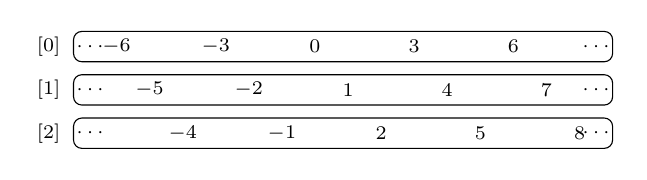
\begin{tikzpicture}[font=\scriptsize, x=0.42cm, y=0.55cm]
\foreach \r in {0,1,2} {
  \draw[line width=0.4pt, rounded corners=3pt] (-0.9,-\r-0.35) rectangle (15.4,-\r+0.35);
  \node[anchor=east] at (-1.0,-\r) {$[\r]$};
  \node at (-0.4,-\r) {$\cdots$};
  \node at (14.9,-\r) {$\cdots$};
  \foreach \c in {0,...,4} {\pgfmathtruncatemacro\v{3*\c-6+\r}\node at (\c*3+\r+0.4,-\r) {$\v$};}}
\end{tikzpicture}}
\caption{Partitions. (A) A set cut into five blocks; two of them are shaded. Each point lies in exactly one block, and ``lying in the same block'' is an equivalence relation whose classes are the blocks. (B) Congruence modulo $3$ partitions $\mathbb Z$ into the three classes $[0]$, $[1]$ and $[2]$; the integers increase from left to right, each in the row of its class.}
\label{fig:partition}
\end{figure}

\subsection{Functions on Quotient Sets}

Equivalence relations arise naturally from functions. If $f\colon A\to B$ is any function, declare two elements of $A$ equivalent when $f$ does not distinguish them:
\[
a\sim_f a'\iff f(a)=f(a').
\]
This relation is reflexive, symmetric and transitive because equality is. Its classes are the nonempty preimages $f^{-1}(\{b\})$, $b\in f(A)$, the sets of inputs that share an output. Congruence modulo $3$ is of this kind, with $f(n)$ the remainder of $n$ on division by $3$, and so is $x^2=y^2$, with $f(x)=x^2$. Conversely, every equivalence relation $\sim$ on $A$ arises in this way: the \term{canonical projection}
\[
\pi\colon A\to A/{\sim},\qquad\pi(a)\coloneqq[a],
\]
is surjective, and $\pi(a)=\pi(a')$ holds if and only if $a\sim a'$, by \cref{lem:classes}\,(ii). So $\sim$ is the relation $\sim_\pi$~\cite{halmos1960naive}.

Grouping the rows of a table by a key is exactly this construction: the key column is a function $f$ on the rows, the groups are the classes of $\sim_f$, and a summary of each group, such as the sum of a numerical column, is a function on the quotient set, as Volume~VII describes.

Defining a function on a quotient set requires care, because a class has many names. Suppose we wish to define $\bar g\colon A/{\sim}\to C$ by the formula $\bar g([a])\coloneqq g(a)$ for some function $g\colon A\to C$. If $[a]=[a']$ with $a\ne a'$, the formula prescribes two values, $g(a)$ and $g(a')$, for the same class, and $\bar g$ is a function only if these values always agree, that is, if
\[
a\sim a'\Rightarrow g(a)=g(a').
\]
A definition that satisfies this condition is called \term{well defined}. For example, on $\mathbb Z/3\mathbb Z$ the rule $[a]\mapsto[a^2]$ is well defined: if $a\equiv a'\pmod3$, say $a'=a+3k$, then $a'^2-a^2=6ak+9k^2=3(2ak+3k^2)$, so $[a'^2]=[a^2]$. The rule $[a]\mapsto a^2$ into $\mathbb Z$ is not well defined, since $[1]=[4]$ but $1^2\ne4^2$. The following theorem uses the condition to show that every function is a composition of three simple ones.

\begin{theorem}[Factorisation of a function]
\label{thm:factorisation}
Let $f\colon A\to B$ be a function, $\sim_f$ the equivalence relation above, $\pi\colon A\to A/{\sim_f}$ the canonical projection and $\iota\colon f(A)\to B$ the inclusion of the range. The rule $\bar f([a])\coloneqq f(a)$ defines a bijection $\bar f\colon A/{\sim_f}\to f(A)$, and
\[
f=\iota\circ\bar f\circ\pi .
\]
\end{theorem}

\begin{proof}
\emph{Well defined.} If $[a]=[a']$, then $a\sim_fa'$, that is, $f(a)=f(a')$. So the value $\bar f([a])$ does not depend on the representative, and $\bar f$ is a function from $A/{\sim_f}$ to $f(A)$.

\emph{Injective.} If $\bar f([a])=\bar f([a'])$, then $f(a)=f(a')$, so $a\sim_fa'$ and $[a]=[a']$.

\emph{Surjective.} Every element of $f(A)$ is $f(a)=\bar f([a])$ for some $a\in A$.

\emph{Factorisation.} For every $a\in A$, $(\iota\circ\bar f\circ\pi)(a)=\iota(\bar f([a]))=f(a)$.
\end{proof}

The theorem says that a function does three things in turn: it merges the inputs it cannot tell apart (the surjection $\pi$), it relabels the resulting classes in a one-to-one manner (the bijection $\bar f$), and it places the labels inside a possibly larger codomain (the injection $\iota$). Versions of this factorisation appear in linear algebra, where it underlies the rank--nullity theorem of Chapter~16, and in algebra generally.

\subsection{Constructing Numbers as Classes}

Equivalence classes also serve to construct new mathematical objects. The fractions $\tfrac12$, $\tfrac24$ and $\tfrac{-3}{-6}$ are different expressions of the same rational number. This suggests defining a rational number as a class of pairs of integers. On the set $\mathbb Z\times(\mathbb Z\setminus\{0\})$ of pairs $(p,q)$ with $q\ne0$, define
\[
(p,q)\sim(r,s)\iff ps=qr .
\]
The condition says that $p/q=r/s$, but it is written without division, so that it uses only the arithmetic of integers.

\begin{proposition}
\label{prop:fractions}
The relation $\sim$ on $\mathbb Z\times(\mathbb Z\setminus\{0\})$ is an equivalence relation.
\end{proposition}

\begin{proof}
Reflexivity: $pq=qp$. Symmetry: if $ps=qr$, then $rq=sp$. Transitivity: suppose $(p,q)\sim(r,s)$ and $(r,s)\sim(t,u)$, that is, $ps=qr$ and $ru=st$. Multiplying the first equation by $u$ and using the second,
\[
psu=qru=qst ,
\]
so $s(pu-qt)=0$. Since $s\ne0$, it follows that $pu=qt$, which is $(p,q)\sim(t,u)$.
\end{proof}

The proof used the hypothesis $s\ne0$, and this is why pairs with second component $0$ were excluded: if the pair $(0,0)$ were allowed, then $(1,1)\sim(0,0)$ and $(0,0)\sim(0,1)$ would hold, since every product involving the pair $(0,0)$ vanishes, while $(1,1)\sim(0,1)$ fails. A rational number can be \emph{defined} as an equivalence class $[(p,q)]$, and addition and multiplication of classes by
\[
[(p,q)]+[(r,s)]\coloneqq[(ps+qr,qs)],\qquad[(p,q)]\cdot[(r,s)]\coloneqq[(pr,qs)],
\]
after checking that these definitions are well defined. Chapter~3 returns to this construction.

\section{Orders}
\label{sec:orders}

Sorting a list, finding the largest entry, choosing the best solution: all of these presuppose a way of comparing elements. The relations that make comparison precise are the orders~\cite{daveypriestley2002}.

\subsection{Partial and Total Orders}

\begin{definition}[Partial order, total order]
\label{def:order}
A \term{partial order} on a set $P$ is a relation $\le$ on $P$ that is reflexive, antisymmetric and transitive. The pair $(P,\le)$ is a \term{partially ordered set}, or \term{poset}. Two elements $a$ and $b$ are \term{comparable} if $a\le b$ or $b\le a$. A partial order in which every two elements are comparable is a \term{total order}, or linear order, and $(P,\le)$ is then a \term{totally ordered set}.
\end{definition}

We use the symbol $\le$ for an arbitrary partial order, write $b\ge a$ for $a\le b$, and write $a<b$ for ``$a\le b$ and $a\ne b$''. By \cref{tab:relation-properties}, the usual order $\le$ on $\mathbb R$ (and on its subsets $\mathbb N$, $\mathbb Z$, $\mathbb Q$) is a partial order, and it is total. Divisibility on $\mathbb N$ and inclusion on $\mathcal P(X)$ are partial orders that are not total: $2$ and $3$ are incomparable under divisibility, since neither divides the other, and $\{1\}$ and $\{2\}$ are incomparable under inclusion. Partial orders that are not total are common. Two tasks in a project, one of which must be finished before the other can begin, are comparable, while two independent tasks are not; vectors in $\mathbb R^2$ compared component by component, $(x_1,y_1)\le(x_2,y_2)$ if $x_1\le x_2$ and $y_1\le y_2$, are not always comparable either.

The strict relation $<$ has its own characterisation, and either of $\le$ and $<$ determines the other.

\begin{proposition}
\label{prop:strict-order}
Let $\le$ be a partial order on $P$ and define $a<b$ if $a\le b$ and $a\ne b$. Then $<$ is \term{irreflexive} (no $a$ satisfies $a<a$) and transitive, and $a\le b$ holds if and only if $a<b$ or $a=b$. Conversely, if $<$ is an irreflexive and transitive relation on $P$, then ``$a<b$ or $a=b$'' defines a partial order on $P$.
\end{proposition}

\begin{proof}
Irreflexivity is immediate from the definition. For transitivity, let $a<b$ and $b<c$. Then $a\le b$ and $b\le c$, so $a\le c$. If $a=c$, then $a\le b$ and $b\le a$, so $a=b$ by antisymmetry, contradicting $a<b$; hence $a\ne c$ and $a<c$. The description of $\le$ in terms of $<$ is the law of excluded middle applied to $a=b$.

For the converse, let $a\le b$ mean ``$a<b$ or $a=b$''. Reflexivity is clear. For antisymmetry, suppose $a\le b$, $b\le a$ and $a\ne b$; then $a<b$ and $b<a$, so $a<a$ by transitivity, which is impossible. For transitivity, if $a\le b$ and $b\le c$, then $a=b$ or $b=c$ gives $a\le c$ at once, and otherwise $a<b<c$ gives $a<c$.
\end{proof}

An irreflexive and transitive relation is called a \term{strict partial order}. In a total order, \term{trichotomy} holds: for every $a$ and $b$ exactly one of $a<b$, $a=b$ and $b<a$ is true.

\subsection{Hasse Diagrams}

The directed graph of a partial order on a finite set, as in \cref{fig:relation}A, is cluttered: every element has a loop, and with arrows from $a$ to $b$ and from $b$ to $c$ there is always an arrow from $a$ to $c$. Since reflexivity and transitivity are known in advance, these arrows carry no information. A \term{Hasse diagram}, named after Helmut Hasse~\cite{daveypriestley2002}, omits them. We say that $b$ \term{covers} $a$ if $a<b$ and there is no $c$ with $a<c<b$. The Hasse diagram draws the elements as points, places $b$ higher than $a$ whenever $a<b$, and joins $a$ and $b$ by a line exactly when $b$ covers $a$. Then $a<b$ holds if and only if one can climb from $a$ to $b$ along lines, always going upwards. \Cref{fig:hasse} shows three examples. In panel C, which is the order of \cref{fig:relation}, the seven arrows between different elements are reduced to five lines, and the loops are gone.

\begin{figure}
\tikzset{hv/.style={circle, fill=black, inner sep=0pt, minimum size=3.4pt},
  hl/.style={line width=0.5pt}}
\sdpanel{A}{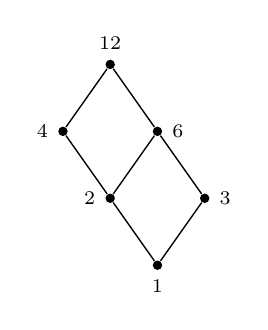
\begin{tikzpicture}[font=\scriptsize]
\node[hv, label=below:$1$] (1) at (0,0) {};
\node[hv, label=left:$2$] (2) at (-0.6,0.85) {};
\node[hv, label=right:$3$] (3) at (0.6,0.85) {};
\node[hv, label=left:$4$] (4) at (-1.2,1.7) {};
\node[hv, label=right:$6$] (6) at (0,1.7) {};
\node[hv, label=above:$12$] (12) at (-0.6,2.55) {};
\draw[hl] (1)--(2) (1)--(3) (2)--(4) (2)--(6) (3)--(6) (4)--(12) (6)--(12);
\end{tikzpicture}}\hfill
\sdpanel{B}{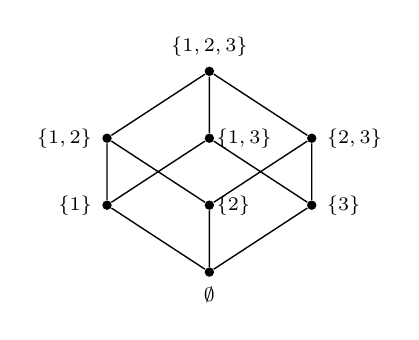
\begin{tikzpicture}[font=\scriptsize]
\node[hv, label={below:$\emptyset$}] (e) at (0,0) {};
\node[hv, label={left:$\{1\}$}] (a) at (-1.3,0.85) {};
\node[hv, label={[fill=white, inner sep=0.5pt]right:$\{2\}$}] (b) at (0,0.85) {};
\node[hv, label={right:$\{3\}$}] (c) at (1.3,0.85) {};
\node[hv, label={left:$\{1,2\}$}] (ab) at (-1.3,1.7) {};
\node[hv, label={[fill=white, inner sep=0.5pt]right:$\{1,3\}$}] (ac) at (0,1.7) {};
\node[hv, label={right:$\{2,3\}$}] (bc) at (1.3,1.7) {};
\node[hv, label={above:$\{1,2,3\}$}] (abc) at (0,2.55) {};
\draw[hl] (e)--(a) (e)--(b) (e)--(c) (a)--(ab) (a)--(ac) (b)--(ab) (b)--(bc) (c)--(ac) (c)--(bc) (ab)--(abc) (ac)--(abc) (bc)--(abc);
\end{tikzpicture}}\hfill
\sdpanel{C}{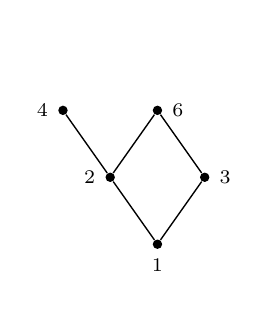
\begin{tikzpicture}[font=\scriptsize]
\node[hv, label=below:$1$] (1) at (0,0) {};
\node[hv, label=left:$2$] (2) at (-0.6,0.85) {};
\node[hv, label=right:$3$] (3) at (0.6,0.85) {};
\node[hv, label=left:$4$] (4) at (-1.2,1.7) {};
\node[hv, label=right:$6$] (6) at (0,1.7) {};
\draw[hl] (1)--(2) (1)--(3) (2)--(4) (2)--(6) (3)--(6);
\path (0,2.55) -- (0,2.75);
\end{tikzpicture}}
\caption{Hasse diagrams. (A) The divisors of $12$ ordered by divisibility. (B) The subsets of $\{1,2,3\}$ ordered by inclusion; the diagram is a cube. (C) The divisors of $12$ other than $12$ itself: there are two maximal elements, $4$ and $6$, and no greatest element.}
\label{fig:hasse}
\end{figure}

\subsection{Greatest, Maximal, and Bounds}

\begin{definition}[Greatest and maximal elements]
\label{def:maximal}
Let $(P,\le)$ be a poset and $S\subseteq P$.
\begin{enumerate}
\item An element $g\in S$ is the \term{greatest element}, or \term{maximum}, of $S$ if $s\le g$ for every $s\in S$. The \term{least element}, or \term{minimum}, is defined with $\ge$ in place of $\le$. We write $\max S$ and $\min S$.
\item An element $m\in S$ is a \term{maximal element} of $S$ if no element of $S$ is strictly greater: there is no $s\in S$ with $m<s$. \term{Minimal elements} are defined in the same way.
\end{enumerate}
\end{definition}

The difference between ``greatest'' and ``maximal'' is the difference between ``above everything'' and ``below nothing''. In \cref{fig:hasse}C the elements $4$ and $6$ are both maximal, since nothing lies above either of them, but neither is greatest, since they are incomparable. In \cref{fig:hasse}A the element $12$ is greatest. The set $\mathcal P(X)$ ordered by inclusion has the greatest element $X$ and the least element $\emptyset$. In the totally ordered set $\mathbb R$ the interval $[0,1)$ has the least element $0$ but neither a greatest nor a maximal element: for every $x\in[0,1)$, the number $(x+1)/2$ lies in $[0,1)$ and is larger than $x$.

\begin{proposition}
\label{prop:maximal}
Let $(P,\le)$ be a poset and $S\subseteq P$.
\begin{enumerate}
\item $S$ has at most one greatest element.
\item A greatest element of $S$ is maximal, and it is the only maximal element of $S$.
\item If $\le$ is a total order, every maximal element of $S$ is greatest.
\item If $S$ is finite and nonempty, $S$ has at least one maximal element and at least one minimal element.
\end{enumerate}
\end{proposition}

\begin{proof}
(i) If $g$ and $g'$ are greatest, then $g'\le g$ and $g\le g'$, so $g=g'$ by antisymmetry.

(ii) Let $g$ be greatest, and suppose $g<s$ for some $s\in S$. Since also $s\le g$, antisymmetry gives $s=g$, contradicting $g<s$; so $g$ is maximal. If $m$ is any maximal element, then $m\le g$, and $m<g$ is impossible by maximality, so $m=g$.

(iii) Let $m$ be maximal and $s\in S$. By totality, $s\le m$ or $m\le s$. In the second case $m<s$ is excluded by maximality, so $m=s$, and $s\le m$ holds in either case.

(iv) We prove the claim for maximal elements by induction on the number $n\ge1$ of elements of $S$; the claim for minimal elements follows by exchanging $\le$ and $\ge$. If $n=1$, the only element is maximal. Let $S$ have $n+1$ elements, choose $x\in S$ and put $S'\coloneqq S\setminus\{x\}$, which has $n$ elements and, by the inductive hypothesis, a maximal element $m'$. If $m'<x$ does not hold, then $m'$ is maximal in $S$: an element $s\in S$ with $m'<s$ would have to be $x$, as $m'$ is maximal in $S'$. If $m'<x$, then $x$ is maximal in $S$: if $x<s$ for some $s\in S$, then $s\ne x$, so $s\in S'$, and $m'<x<s$ contradicts the maximality of $m'$ in $S'$.
\end{proof}

Part (iv) has a useful consequence. A task schedule is a partial order on a finite set of tasks, and a valid sequence in which to perform the tasks is a total order that is compatible with it. Such a sequence always exists.

\begin{theorem}[Linear extensions]
\label{thm:linear-extension}
Let $\le$ be a partial order on a finite set $P$ with $n$ elements. Then the elements of $P$ can be listed as $p_1,p_2,\ldots,p_n$ in such a way that $p_i<p_j$ implies $i<j$.
\end{theorem}

\begin{proof}
We use induction on $n$; for $n=0$ the empty list will do. Let $P$ have $n+1$ elements. By \cref{prop:maximal}\,(iv), $P$ has a minimal element; call it $p_1$. The set $P\setminus\{p_1\}$, with the same order, has $n$ elements, and by the inductive hypothesis it can be listed as $p_2,\ldots,p_{n+1}$ with the required property. In the combined list, suppose $p_i<p_j$. If $i,j\ge2$, then $i<j$ by the construction of the shorter list. The case $j=1$ is impossible, because $p_1$ is minimal. If $i=1$, then $j\ne1$, since $p_1<p_1$ is false, so $1<j$.
\end{proof}

Listing the elements as in the theorem defines a total order that extends the given partial order. For the divisors of $12$ in \cref{fig:hasse}A, both $1,2,3,4,6,12$ and $1,3,2,6,4,12$ are such lists. Szpilrajn proved that every partial order, even on an infinite set, can be extended to a total order~\cite{szpilrajn1930}; for infinite sets the proof needs the axiom of choice. The proof above is an algorithm in disguise: repeatedly remove a minimal element. Its efficient implementation is called \term{topological sorting}, and Volume~IV presents it as an algorithm on directed graphs.

Maximal and greatest elements are found inside a set. Bounds may lie outside it.

\begin{definition}[Bounds, supremum, infimum]
\label{def:sup}
Let $(P,\le)$ be a poset and $S\subseteq P$. An element $u\in P$ is an \term{upper bound} of $S$ if $s\le u$ for every $s\in S$, and a \term{lower bound} if $u\le s$ for every $s\in S$. The set $S$ is \term{bounded above} if it has an upper bound, and \term{bounded below} if it has a lower bound. If the set of upper bounds of $S$ has a least element, this element is the \term{supremum}, or least upper bound, of $S$, written $\sup S$. If the set of lower bounds has a greatest element, it is the \term{infimum}, or greatest lower bound, written $\inf S$.
\end{definition}

By \cref{prop:maximal}\,(i), a set has at most one supremum and at most one infimum, which justifies the notation. If $S$ has a greatest element $g$, then $g$ is an upper bound that belongs to $S$, so every upper bound $u$ satisfies $g\le u$, and $g=\sup S$. The supremum is the right replacement for the maximum when the maximum does not exist.

\begin{proposition}
\label{prop:sup-interval}
In $\mathbb R$ with its usual order, $\sup{[0,1)}=1$, although $[0,1)$ has no greatest element.
\end{proposition}

\begin{proof}
The number $1$ is an upper bound of $[0,1)$. Let $u$ be any upper bound; we show $1\le u$. Suppose, for a contradiction, that $u<1$. Since $0\in[0,1)$, we have $u\ge0$. The number $x\coloneqq(u+1)/2$ satisfies $0\le u<x<1$, so $x\in[0,1)$, and $x>u$ contradicts the assumption that $u$ is an upper bound. Hence $1$ is the least upper bound. We showed above that $[0,1)$ has no greatest element.
\end{proof}

In other posets the supremum takes other forms. In $\mathcal P(X)$ ordered by inclusion, $\sup\{A,B\}=A\cup B$ and $\inf\{A,B\}=A\cap B$, because $A\cup B$ contains both $A$ and $B$ and is contained in every set that contains both, and dually for $A\cap B$. In $\mathbb N$ ordered by divisibility, $\inf\{4,6\}=2$ and $\sup\{4,6\}=12$: the lower bounds of $\{4,6\}$ are the common divisors $1$ and $2$, and the upper bounds are the common multiples $0,12,24,\ldots$, among which $12$ divides all the others. In general the infimum and supremum of two natural numbers under divisibility are their greatest common divisor and least common multiple, as Chapter~3 shows. In this order $0$ is the greatest element of $\mathbb N$, since every natural number divides $0$.

A supremum need not exist. In $\mathbb Q$ with its usual order, the set $\{q\in\mathbb Q: q^2<2\}$ is bounded above, for instance by $2$, but it has no least upper bound in $\mathbb Q$: the candidate would be $\sqrt2$, which is not rational. The property that distinguishes $\mathbb R$ from $\mathbb Q$ is precisely that every nonempty subset of $\mathbb R$ that is bounded above has a supremum in $\mathbb R$. This is the completeness axiom, on which Chapter~3 bases the theory of the real numbers and much of calculus rests.

\subsection{Lexicographic Order}

Dictionaries order words by their first letter, words with the same first letter by their second letter, and so on. The same principle orders pairs and tuples.

\begin{definition}[Lexicographic order]
\label{def:lex}
Let $(A,\le_A)$ and $(B,\le_B)$ be posets. The \term{lexicographic order} on $A\times B$ is defined by
\[
(a,b)\le_{\mathrm{lex}}(a',b')\iff a<_Aa'\ \vee\ \bigl(a=a'\wedge b\le_Bb'\bigr).
\]
\end{definition}

The first components decide, and the second components are consulted only when the first components are equal. For example, in $\mathbb N\times\mathbb N$,
\[
(0,5)<_{\mathrm{lex}}(1,0)<_{\mathrm{lex}}(1,3)<_{\mathrm{lex}}(2,0).
\]

\begin{proposition}
\label{prop:lex}
If $\le_A$ and $\le_B$ are partial orders, then $\le_{\mathrm{lex}}$ is a partial order on $A\times B$. If both are total, so is $\le_{\mathrm{lex}}$.
\end{proposition}

\begin{proof}
Reflexivity: $(a,b)\le_{\mathrm{lex}}(a,b)$ because $a=a$ and $b\le_Bb$.

Antisymmetry: suppose $(a,b)\le_{\mathrm{lex}}(a',b')$ and $(a',b')\le_{\mathrm{lex}}(a,b)$. If $a\ne a'$, the two relations would give $a<_Aa'$ and $a'<_Aa$, hence $a<_Aa$ by \cref{prop:strict-order}, which is impossible. So $a=a'$, and then $b\le_Bb'$ and $b'\le_Bb$ give $b=b'$.

Transitivity: suppose $(a,b)\le_{\mathrm{lex}}(a',b')$ and $(a',b')\le_{\mathrm{lex}}(a'',b'')$. Then $a\le_Aa'\le_Aa''$, so $a\le_Aa''$. If $a<_Aa''$, we are done. Otherwise $a=a''$, and antisymmetry applied to $a\le_Aa'\le_Aa''=a$ gives $a=a'=a''$. Then both relations are decided by the second components, $b\le_Bb'\le_Bb''$, and $(a,b)\le_{\mathrm{lex}}(a'',b'')$.

Totality: let $(a,b)$ and $(a',b')$ be given, with $\le_A$ and $\le_B$ total. By trichotomy in $A$, either $a<_Aa'$, or $a'<_Aa$, or $a=a'$. In the first two cases the pairs are comparable by their first components, and in the third by their second components, which are comparable because $\le_B$ is total.
\end{proof}

The lexicographic order extends to $n$-tuples: compare the first components, then the second, and so on, stopping at the first position where the tuples differ. It extends also to \term{words}, the finite sequences of letters from an ordered alphabet, with the convention that a word comes before every longer word that begins with it; thus ``set'' $<$ ``sets'' $<$ ``setting''. This is the order in which computers sort strings, and it is the order used when a table is sorted by several columns: the rows are compared by the first key, ties are broken by the second key, and so on~\cite{knuth1998taocp3}. Volumes~VI and~VII rely on it. Sorting rows by a key is, strictly speaking, sorting by a relation that is not antisymmetric: two different rows with the same key are tied. The relation ``the key of $r$ is at most the key of $r'$'' is reflexive, transitive and total but not antisymmetric, and such a relation is called a \term{total preorder}. The ties are exactly the classes of the equivalence relation ``has the same key'' of \cref{sec:equivalence}.

\subsection{Well-Orders}

\begin{definition}[Well-order]
\label{def:well-order}
A total order $\le$ on a set $P$ is a \term{well-order} if every nonempty subset of $P$ has a least element.
\end{definition}

The well-ordering principle (\cref{thm:well-ordering}) states that $\mathbb N$ with its usual order is well-ordered, and this property is what makes induction and the method of the smallest counterexample work. The usual order on $\mathbb Z$ is not a well-order, since $\mathbb Z$ itself has no least element; nor is the usual order on $[0,1]$, since the subset $(0,1]$ has no least element. Every finite totally ordered set is well-ordered: by \cref{prop:maximal}\,(iv) a nonempty subset has a minimal element, and by \cref{prop:maximal}\,(iii), applied with $\ge$ in place of $\le$, a minimal element of a totally ordered set is its least element.

\begin{proposition}
\label{prop:lex-well-order}
If $\le_A$ and $\le_B$ are well-orders, then the lexicographic order on $A\times B$ is a well-order. In particular $\mathbb N\times\mathbb N$ is well-ordered lexicographically.
\end{proposition}

\begin{proof}
By \cref{prop:lex}, $\le_{\mathrm{lex}}$ is a total order. Let $S\subseteq A\times B$ be nonempty. The set $S_1\coloneqq\{a\in A:\exists b\in B,\ (a,b)\in S\}$ of first components is nonempty, so it has a least element $a_0$. The set $S_2\coloneqq\{b\in B: (a_0,b)\in S\}$ is nonempty, by the choice of $a_0$, so it has a least element $b_0$. We claim that $(a_0,b_0)$ is the least element of $S$. It lies in $S$. Let $(a,b)\in S$. Then $a\in S_1$, so $a_0\le_Aa$. If $a_0<_Aa$, then $(a_0,b_0)<_{\mathrm{lex}}(a,b)$. If $a=a_0$, then $b\in S_2$, so $b_0\le_Bb$ and $(a_0,b_0)\le_{\mathrm{lex}}(a,b)$.
\end{proof}

The lexicographic well-order on $\mathbb N\times\mathbb N$ differs from that of $\mathbb N$ in an instructive way. The element $(1,0)$ is preceded by infinitely many elements, all the pairs $(0,n)$, whereas every natural number has only finitely many predecessors. A loop that decreases a pair $(a,b)\in\mathbb N^2$ lexicographically at every pass must stop, by the argument of \cref{prop:tobinary} with \cref{prop:lex-well-order} in place of \cref{thm:well-ordering}, even though $b$ may increase without bound whenever $a$ decreases. Termination proofs of this kind appear in Volume~IV.

\subsection{Comparisons That Are Not Orders}

Algorithms that sort, search or find a maximum use only comparisons, and they assume that the comparison is a total order, or at least a total preorder. When this assumption fails, they fail too, often silently. Suppose a list contains the numbers $3$ and $1$ and a special value $u$ that, by convention, is neither smaller nor larger than any number and not equal to any number either. Consider the list $(3,u,1)$. A test that a list is sorted typically checks only adjacent entries. Here $u<3$ is false and $1<u$ is false, so no adjacent pair is out of order, and the test accepts the list, although $3>1$. The test is valid only if from ``$3$ is not greater than $u$'' and ``$u$ is not greater than $1$'' one may conclude ``$3$ is not greater than $1$''. That conclusion relies on the transitivity of the relation ``is not greater than'', and transitivity fails once $u$ is present. Depending on the order of the input, a sorting algorithm may therefore leave $3$ before $1$ or after it, and different algorithms disagree. Floating-point arithmetic contains a value with exactly this behaviour, as Volume~V explains, and Volume~VI describes how sorting routines treat it to obtain a well-defined result.

\section{Cardinality}
\label{sec:cardinality}

To count the elements of a finite set is to pair them off with the numbers $1,2,\ldots,n$, or, in the convention of this series, with $0,1,\ldots,n-1$. In the language of \cref{sec:injections}, counting is the construction of a bijection. This point of view, due to Cantor, makes sense for infinite sets as well, and it leads to the discovery that infinite sets come in different sizes~\cite{cantor1874,cantor1891}.

\subsection{Equinumerous Sets}

\begin{definition}[Equinumerous sets]
\label{def:equinumerous}
Sets $A$ and $B$ are \term{equinumerous}, or have the same \term{cardinality}, written $|A|=|B|$, if there is a bijection from $A$ to $B$.
\end{definition}

The notation $|A|=|B|$ does not presuppose that $|A|$ is a number; it is a statement about $A$ and $B$, defined as a whole. It behaves like an equality.

\begin{proposition}
\label{prop:equinumerous}
For all sets $A$, $B$ and $C$: $|A|=|A|$; if $|A|=|B|$, then $|B|=|A|$; and if $|A|=|B|$ and $|B|=|C|$, then $|A|=|C|$.
\end{proposition}

\begin{proof}
The identity $\operatorname{id}_A$ is a bijection. If $f\colon A\to B$ is a bijection, so is $f^{-1}\colon B\to A$, by \cref{thm:inverse}. If $f\colon A\to B$ and $g\colon B\to C$ are bijections, so is $g\circ f$, by \cref{prop:composition-injective}\,(iii).
\end{proof}

For infinite sets the definition has unexpected consequences. The map $n\mapsto n+1$ is a bijection from $\mathbb N$ to $\mathbb N\setminus\{0\}$, and $n\mapsto2n$ is a bijection from $\mathbb N$ to the even natural numbers. So $\mathbb N$ has as many elements as some of its proper subsets, something that no finite set can do, as we show below. Dedekind took this property as the definition of an infinite set~\cite{dedekind1888}. Intervals of real numbers give another example. For real numbers $a<b$, the map $x\mapsto(2x-a-b)/(b-a)$ is a bijection from $(a,b)$ to $(-1,1)$, with inverse $y\mapsto\bigl((b-a)y+a+b\bigr)/2$. More surprisingly, the open interval $(-1,1)$ is equinumerous with the whole real line:
\[
\varphi\colon(-1,1)\to\mathbb R,\qquad\varphi(x)\coloneqq\frac{x}{1-|x|},
\]
is a bijection. To prove this with \cref{thm:inverse}, consider $\psi\colon\mathbb R\to(-1,1)$, $\psi(y)\coloneqq y/(1+|y|)$, which indeed takes values in $(-1,1)$ because $|\psi(y)|=|y|/(1+|y|)<1$. For $y\in\mathbb R$ we have $1-|\psi(y)|=1/(1+|y|)$, and therefore $\varphi(\psi(y))=\frac{y}{1+|y|}\cdot(1+|y|)=y$. For $x\in(-1,1)$ we have $1+|\varphi(x)|=1/(1-|x|)$, and therefore $\psi(\varphi(x))=x$. So $\psi$ is an inverse of $\varphi$. Hence every open interval, however short, has as many points as the whole line.

\subsection{Finite Sets}

\begin{definition}[Finite and infinite sets]
\label{def:finite}
A set $A$ is \term{finite} with $n$ elements, for $n\in\mathbb N$, if $|A|=|\{0,1,\ldots,n-1\}|$; we then write $|A|=n$. (For $n=0$ the set $\{0,\ldots,n-1\}$ is empty.) A set that is not finite is \term{infinite}.
\end{definition}

For this definition to be sensible, a set must not have two different numbers of elements. This, and much more, follows from the next lemma~\cite{hrbacek1999}, which is a form of the pigeonhole principle of Chapter~4: $m$ pigeons cannot be placed in $n<m$ holes, one pigeon per hole.

\begin{lemma}
\label{lem:pigeonhole}
Let $m,n\in\mathbb N$. If there is an injection from $\{0,\ldots,m-1\}$ to $\{0,\ldots,n-1\}$, then $m\le n$.
\end{lemma}

\begin{proof}
We use induction on $n$; the statement $P(n)$ is ``for every $m\in\mathbb N$, if there is an injection from $\{0,\ldots,m-1\}$ to $\{0,\ldots,n-1\}$, then $m\le n$''. For $n=0$ the codomain is empty, and a function into the empty set exists only on the empty domain, so $m=0$.

Assume $P(n)$, and let $f$ be an injection from $\{0,\ldots,m-1\}$ to $\{0,\ldots,n\}$. If $m=0$, then $m\le n+1$. Otherwise, let $\tau$ be the permutation of $\{0,\ldots,n\}$ that exchanges $f(m-1)$ and $n$ and fixes every other element (the identity if $f(m-1)=n$), and put $h\coloneqq\tau\circ f$. Then $h$ is injective by \cref{prop:composition-injective}\,(i), and $h(m-1)=n$. For $i<m-1$, injectivity gives $h(i)\ne h(m-1)=n$, so the restriction of $h$ to $\{0,\ldots,m-2\}$ is an injection into $\{0,\ldots,n-1\}$. By $P(n)$, $m-1\le n$, that is, $m\le n+1$.
\end{proof}

\begin{corollary}
\label{cor:finite}
\leavevmode
\begin{enumerate}
\item If $|A|=m$ and $|A|=n$, then $m=n$.
\item The set $\mathbb N$ is infinite.
\item Let $A$ be finite. A function $f\colon A\to A$ is injective if and only if it is surjective.
\end{enumerate}
\end{corollary}

\begin{proof}
(i) Composing a bijection from $\{0,\ldots,m-1\}$ to $A$ with a bijection from $A$ to $\{0,\ldots,n-1\}$ gives a bijection, so $m\le n$ by \cref{lem:pigeonhole}; by symmetry $n\le m$.

(ii) Suppose $g\colon\mathbb N\to\{0,\ldots,n-1\}$ were a bijection for some $n$. Its restriction to $\{0,\ldots,n\}$ would be an injection into $\{0,\ldots,n-1\}$, so $n+1\le n$ by \cref{lem:pigeonhole}, which is false.

(iii) Let $|A|=n$. Transporting $f$ along a bijection between $A$ and $\{0,\ldots,n-1\}$ does not change injectivity or surjectivity, by \cref{prop:composition-injective}, so we may assume $A=\{0,\ldots,n-1\}$, and we may assume $n\ge1$, as the case $n=0$ is trivial. Suppose $f$ is injective but not surjective, and let $b$ be an element not in its range. Let $\tau$ exchange $b$ and $n-1$. Then $\tau\circ f$ is injective and never takes the value $n-1$, so it is an injection from $\{0,\ldots,n-1\}$ to $\{0,\ldots,n-2\}$, which contradicts \cref{lem:pigeonhole}. Hence injective functions are surjective. Now suppose $f$ is surjective. Let $g(b)$ be the least element of $f^{-1}(\{b\})$; then $f\circ g=\operatorname{id}_A$, so $g$ is injective by \cref{prop:composition-injective}\,(iv), hence surjective by what we have just proved, hence bijective. Then $f=f\circ g\circ g^{-1}=g^{-1}$ is bijective, in particular injective.
\end{proof}

In particular, a finite set $A$ is never equinumerous with a proper subset $B\subset A$, as promised above: a bijection from $A$ to $B$, regarded as a function from $A$ to $A$, would be injective but not surjective, contradicting (iii). Part (iii) fails for infinite sets: $n\mapsto n+1$ is an injection of $\mathbb N$ into itself that is not surjective, and the halving function of \cref{sec:injections} is a surjection that is not injective. Part (iii) is often used to establish bijectivity with half the work, and Part~III uses its linear-algebra analogue for square matrices.

\subsection{Countable Sets}

\begin{definition}[Countable and uncountable sets]
\label{def:countable}
A set $A$ is \term{countably infinite} if $|A|=|\mathbb N|$, \term{countable} if it is finite or countably infinite, and \term{uncountable} if it is not countable.
\end{definition}

A countably infinite set is one whose elements can be arranged in an infinite list $a_0,a_1,a_2,\ldots$ in which every element appears exactly once: the bijection $f\colon\mathbb N\to A$ is the list, with $a_n=f(n)$. The examples above show that $\mathbb N\setminus\{0\}$ and the even natural numbers are countably infinite. Every subset of $\mathbb N$ is countable, and the proof shows how to list it.

\begin{lemma}
\label{lem:subset-n}
Every subset $S$ of $\mathbb N$ is countable. More precisely, either $S$ is finite, or the elements of $S$ in increasing order $a_0<a_1<a_2<\cdots$ form a bijection $k\mapsto a_k$ from $\mathbb N$ to $S$.
\end{lemma}

\begin{proof}
Define $a_0,a_1,\ldots$ recursively: as long as the set $S_k\coloneqq S\setminus\{a_0,\ldots,a_{k-1}\}$ is nonempty, let $a_k$ be its least element, which exists by \cref{thm:well-ordering}. If $S_k=\emptyset$ for some $k$, then $S=\{a_0,\ldots,a_{k-1}\}$, and since the $a_i$ are different by construction, $i\mapsto a_i$ is a bijection from $\{0,\ldots,k-1\}$ to $S$; so $S$ is finite.

Otherwise $a_k$ is defined for every $k\in\mathbb N$. Since $a_{k+1}\in S_{k+1}\subseteq S_k$ and $a_k=\min S_k$, we have $a_k\le a_{k+1}$, and $a_k\ne a_{k+1}$ by construction; so $a_k<a_{k+1}$. Hence $k\mapsto a_k$ is strictly increasing and in particular injective, and $a_k\ge k$ for every $k$, by induction. For surjectivity, let $s\in S$ and suppose that $s\notin\{a_0,\ldots,a_s\}$. Then $s\in S_k$ for every $k\le s$, so $a_k=\min S_k\le s$, and $a_k\ne s$, so $a_k<s$. In particular $a_s<s$, contradicting $a_s\ge s$. Hence $s=a_k$ for some $k\le s$.
\end{proof}

\begin{corollary}
\label{cor:countable}
\leavevmode
\begin{enumerate}
\item A set $A$ is countable if and only if there is an injection from $A$ to $\mathbb N$.
\item A nonempty set $A$ is countable if and only if there is a surjection from $\mathbb N$ to $A$.
\item Every subset of a countable set is countable, and every subset of a finite set is finite.
\end{enumerate}
\end{corollary}

\begin{proof}
(i) If $A$ is countable, a bijection from $A$ to $\mathbb N$ or to some $\{0,\ldots,n-1\}\subseteq\mathbb N$ is an injection into $\mathbb N$. Conversely, an injection $f\colon A\to\mathbb N$ is a bijection from $A$ onto its range $f(A)$, which is countable by \cref{lem:subset-n}; by \cref{prop:equinumerous}, $A$ is countable.

(ii) If $A$ is countably infinite, a bijection $\mathbb N\to A$ is a surjection. If $A=\{a_0,\ldots,a_{n-1}\}$ is finite with $n\ge1$, then $k\mapsto a_k$ for $k<n$ and $k\mapsto a_0$ for $k\ge n$ is a surjection. Conversely, let $g\colon\mathbb N\to A$ be surjective, and let $h(a)$ be the least element of the nonempty set $g^{-1}(\{a\})$. Then $g\circ h=\operatorname{id}_A$, so $h\colon A\to\mathbb N$ is injective by \cref{prop:composition-injective}\,(iv), and $A$ is countable by (i).

(iii) If $B\subseteq A$ and $f\colon A\to\mathbb N$ is injective, then so is $f|_B$, and (i) applies. Now let $A$ be finite with $n$ elements, $\varphi\colon A\to\{0,\ldots,n-1\}$ a bijection and $B\subseteq A$. The set $\varphi(B)\subseteq\mathbb N$ is countable by \cref{lem:subset-n}. If it were infinite, a bijection from $\mathbb N$ to $\varphi(B)$, restricted to $\{0,\ldots,n\}$, would be an injection into $\{0,\ldots,n-1\}$, contradicting \cref{lem:pigeonhole}. So $\varphi(B)$ is finite, and so is $B$, which is equinumerous with it.
\end{proof}

With these tools, countability can be established by constructing an injection into $\mathbb N$, which is usually much easier than constructing a bijection.

\begin{proposition}
\label{prop:countable-examples}
\leavevmode
\begin{enumerate}
\item The set $\mathbb Z$ is countably infinite.
\item The map $p\colon\mathbb N\times\mathbb N\to\mathbb N$, $p(m,n)\coloneqq2^m(2n+1)-1$, is a bijection; in particular $\mathbb N\times\mathbb N$ is countably infinite.
\item If $A$ and $B$ are countable, so is $A\cup B$.
\end{enumerate}
\end{proposition}

\begin{proof}
(i) Define $g\colon\mathbb N\to\mathbb Z$ by $g(n)\coloneqq n/2$ for even $n$ and $g(n)\coloneqq-(n+1)/2$ for odd $n$, so that $g$ lists the integers as $0,-1,1,-2,2,\ldots$. The map $z\mapsto2z$ for $z\ge0$ and $z\mapsto-2z-1$ for $z<0$ is an inverse of $g$: for $n=2k$ we get $g(n)=k\ge0$ and then $2k=n$; for $n=2k+1$ we get $g(n)=-(k+1)<0$ and then $2(k+1)-1=n$; and conversely, for $z\ge0$ the even number $2z$ is mapped back to $z$, and for $z<0$ the odd number $-2z-1=2(-z-1)+1$ is mapped back to $-(-2z)/2=z$. By \cref{thm:inverse}, $g$ is a bijection.

(ii) \emph{Injective.} Suppose $2^m(2n+1)=2^{m'}(2n'+1)$, and suppose $m<m'$. Dividing by $2^m$ gives $2n+1=2^{m'-m}(2n'+1)$, whose left side is odd and whose right side is even, which contradicts \cref{prop:parity}. By symmetry $m>m'$ is impossible as well, so $m=m'$, and dividing by $2^m$ gives $2n+1=2n'+1$, so $n=n'$. \emph{Surjective.} We show by strong induction on $N\ge1$ that $N=2^m(2n+1)$ for some $m,n\in\mathbb N$; then $N-1=p(m,n)$, and every natural number is of the form $N-1$. If $N$ is odd, take $m=0$. If $N$ is even, then $N=2N'$ with $1\le N'<N$; by the inductive hypothesis $N'=2^{m'}(2n+1)$, and $N=2^{m'+1}(2n+1)$.

(iii) Let $f\colon A\to\mathbb N$ and $g\colon B\to\mathbb N$ be injections. Define $h\colon A\cup B\to\mathbb N$ by $h(x)\coloneqq2f(x)$ for $x\in A$ and $h(x)\coloneqq2g(x)+1$ for $x\in B\setminus A$. Two elements of $A$ with the same value have the same value under $f$, and are therefore equal; the same holds for two elements of $B\setminus A$ with $g$; and an element of $A$ and one of $B\setminus A$ have values of different parity. So $h$ is injective, and $A\cup B$ is countable by \cref{cor:countable}\,(i).
\end{proof}

By induction, (iii) extends to unions of finitely many countable sets. It extends even to the union of a countable family of countable sets, but the proof must choose a listing for each set of the family, and it uses the axiom of choice~\cite{jech2003}.

\begin{theorem}[Countability of the rational numbers]
\label{thm:q-countable}
The set $\mathbb Q$ is countably infinite.
\end{theorem}

\begin{proof}
For a rational number $r$, the set of positive integers $s$ such that $rs$ is an integer is nonempty, and we let $s(r)$ be its least element, as in the proof of \cref{lem:lowest-terms}. Then $t(r)\coloneqq r\,s(r)$ is an integer, and $r=t(r)/s(r)$. Let $g\colon\mathbb N\to\mathbb Z$ be the bijection of \cref{prop:countable-examples}\,(i) and $p$ the bijection of part (ii), and define
\[
F\colon\mathbb Q\to\mathbb N,\qquad F(r)\coloneqq p\bigl(g^{-1}(t(r)),\,s(r)\bigr).
\]
If $F(r)=F(r')$, then, as $p$ and $g^{-1}$ are injective, $t(r)=t(r')$ and $s(r)=s(r')$, so $r=t(r)/s(r)=r'$. Hence $F$ is injective, and $\mathbb Q$ is countable by \cref{cor:countable}\,(i). It is infinite because it contains the infinite set $\mathbb N$ (\cref{cor:finite}\,(ii) and \cref{cor:countable}\,(iii)).
\end{proof}

The proof is short but not very illuminating. A picture shows better why the rational numbers can be listed although between any two of them there are infinitely many others. Write the positive fractions $p/q$ in an infinite grid, with $p$ indicating the column and $q$ the row, and run through the grid along the diagonals $p+q=2,3,4,\ldots$, each of which is finite, skipping every fraction whose value has appeared before (\cref{fig:rationals}). This produces the list
\[
1,\ \tfrac12,\ 2,\ \tfrac13,\ 3,\ \tfrac14,\ \tfrac23,\ \tfrac32,\ 4,\ \tfrac15,\ 5,\ \tfrac16,\ \tfrac25,\ \tfrac34,\ \tfrac43,\ \tfrac52,\ 6,\ \ldots
\]
in which every positive rational number appears exactly once, at a finite position. Inserting $0$ at the front and following each positive number by its negative gives a list of all of $\mathbb Q$. Cantor's first paper on set theory proved more: even the set of algebraic numbers, the real roots of polynomials with integer coefficients, is countable~\cite{cantor1874}.

\begin{figure}
\sdfloat{%
\begin{tikzpicture}[font=\small, x=1.0cm, y=0.7cm,
  arr/.style={-{Latex[length=1.3mm]}, line width=0.4pt, shorten >=9.5pt, shorten <=9.5pt}]
\foreach \q in {1,...,5} \foreach \p in {1,...,5} {
  \pgfmathtruncatemacro\s{\p+\q}
  \pgfmathtruncatemacro\g{gcd(\p,\q)}
  \ifnum\s<7 \ifnum\g=1 \node at (\p,-\q) {$\p/\q$};
    \else \node[black!40] at (\p,-\q) {$\p/\q$};\fi
  \else \node[black!40] at (\p,-\q) {$\p/\q$};\fi}
\foreach \p in {1,...,5} {\node[black!60, font=\scriptsize] at (\p,-0.3) {$p=\p$};}
\foreach \q in {1,...,5} {\node[black!60, font=\scriptsize, anchor=east] at (0.5,-\q) {$q=\q$};}
\draw[arr] (1,-2) -- (2,-1);
\draw[arr] (1,-3) -- (2,-2); \draw[arr] (2,-2) -- (3,-1);
\draw[arr] (1,-4) -- (2,-3); \draw[arr] (2,-3) -- (3,-2); \draw[arr] (3,-2) -- (4,-1);
\draw[arr] (1,-5) -- (2,-4); \draw[arr] (2,-4) -- (3,-3); \draw[arr] (3,-3) -- (4,-2); \draw[arr] (4,-2) -- (5,-1);
\node at (5.55,-5.5) {$\ddots$};
\end{tikzpicture}}{Listing the positive rational numbers. The fractions $p/q$ are traversed diagonal by diagonal, $p+q=2,3,4,\ldots$, each diagonal from bottom left to top right (arrows). Grey fractions on these diagonals are skipped because their value has already appeared, such as $2/2=1/1$ and $4/2=2/1$; the grey fractions in the lower right corner are reached on later diagonals.\label{fig:rationals}}
\end{figure}

The same method lists all finite texts. An \term{alphabet} is a finite nonempty set $\Sigma$, whose elements are called letters, and a \term{word} over $\Sigma$ is a finite sequence of letters, the empty word included. The set of all words is denoted $\Sigma^*$.

\begin{proposition}
\label{prop:words-countable}
For every alphabet $\Sigma$, the set $\Sigma^*$ of words is countably infinite.
\end{proposition}

\begin{proof}
Let $c\colon\Sigma\to\mathbb N$ be an injection, which exists because $\Sigma$ is finite, and let $p$ be the bijection of \cref{prop:countable-examples}\,(ii). Define $\kappa\colon\Sigma^*\to\mathbb N$ recursively by the length of the word: $\kappa$ of the empty word is $0$, and if $w$ is a word and $\sigma$ a letter, then $\kappa(w\sigma)\coloneqq p\bigl(\kappa(w),c(\sigma)\bigr)+1$, where $w\sigma$ is $w$ followed by $\sigma$. Thus $\kappa(w)=0$ exactly for the empty word. We show by induction on $n$ that a word $w$ of length $n$ satisfies $\kappa(w)=\kappa(w')$ only for $w'=w$. For $n=0$ this was just observed. If $w=v\sigma$ has length $n+1$ and $\kappa(w')=\kappa(w)\ge1$, then $w'=v'\sigma'$ is not empty, and $p(\kappa(v),c(\sigma))=p(\kappa(v'),c(\sigma'))$. Since $p$ and $c$ are injective, $\kappa(v)=\kappa(v')$ and $\sigma=\sigma'$, and the inductive hypothesis for $v$, which has length $n$, gives $v=v'$. So $\kappa$ is injective and $\Sigma^*$ is countable. It is infinite, because for a letter $\sigma$ the words $\sigma$, $\sigma\sigma$, $\sigma\sigma\sigma$, \ldots\ are all different.
\end{proof}

A more intuitive listing orders the words first by length and then, within each length, lexicographically (\cref{sec:orders}). Over the alphabet $\{a,b\}$ it begins with the empty word, then $a$, $b$, $aa$, $ab$, $ba$, $bb$, $aaa$, and so on; each word appears at a finite position, because only finitely many words are shorter than it or have the same length. The proposition has a consequence for computing. Every program, in any programming language, is a finite text over a finite alphabet, and so the set of all programs is countable. The same holds for every finite description of a number, by a formula or otherwise.

\subsection{Uncountable Sets}

Are all infinite sets countable? Cantor showed in 1874 that the real numbers are not~\cite{cantor1874}. The argument that we give is his later \term{diagonal argument} of 1891~\cite{cantor1891}, which is simpler and applies far more widely. We first apply it to infinite sequences of zeros and ones.

\begin{theorem}
\label{thm:binary-sequences}
The set $\{0,1\}^{\mathbb N}$ of all infinite sequences of zeros and ones is uncountable.
\end{theorem}

\begin{proof}
Let $s\colon\mathbb N\to\{0,1\}^{\mathbb N}$ be any function, and write $s_k$ for the sequence $s(k)$ and $s_k(j)$ for its $j$th term. Define a sequence $d$ by
\[
d(k)\coloneqq1-s_k(k)\qquad(k\in\mathbb N).
\]
For every $k$, the sequences $d$ and $s_k$ differ in their $k$th terms, one being $0$ and the other $1$, so $d\ne s_k$. Hence $d$ is not in the range of $s$, and no function from $\mathbb N$ to $\{0,1\}^{\mathbb N}$ is surjective. Since $\{0,1\}^{\mathbb N}$ is nonempty, it is not countable, by \cref{cor:countable}\,(ii).
\end{proof}

The name of the argument comes from the picture in \cref{tab:diagonal}. If the sequences $s_0,s_1,s_2,\ldots$ are written as the rows of an infinite table, the terms $s_k(k)$ lie on its diagonal, and $d$ is the diagonal with every digit flipped. Whatever list we start from, the flipped diagonal escapes it.

\begin{table}
\sdfloat{%
\begin{sdtable}{colspec={lccccccc}, row{1}={font=\small}, row{8}={font=\small}}
\toprule
 & $j=0$ & $1$ & $2$ & $3$ & $4$ & $5$ & $\cdots$ \\
\midrule
$s_0$ & $\mathbf 0$ & 1 & 0 & 1 & 0 & 1 & $\cdots$ \\
$s_1$ & 1 & $\mathbf 1$ & 1 & 1 & 1 & 1 & $\cdots$ \\
$s_2$ & 0 & 0 & $\mathbf 0$ & 0 & 0 & 0 & $\cdots$ \\
$s_3$ & 1 & 0 & 0 & $\mathbf 1$ & 1 & 0 & $\cdots$ \\
$s_4$ & 0 & 1 & 1 & 0 & $\mathbf 1$ & 0 & $\cdots$ \\
$s_5$ & 1 & 1 & 0 & 0 & 0 & $\mathbf 1$ & $\cdots$ \\
\midrule
$d$ & 1 & 0 & 1 & 0 & 0 & 0 & $\cdots$ \\
\bottomrule
\end{sdtable}}{The diagonal argument. The rows are the first terms of a list of sequences $s_0,s_1,\ldots$; the diagonal terms $s_k(k)$ are set in bold. The sequence $d$ flips each diagonal term and therefore differs from every $s_k$ in position $k$.\label{tab:diagonal}}
\end{table}

To pass from sequences to real numbers, we read a sequence of zeros and ones as the digits of a decimal number. We use two facts about infinite series that are proved in Chapter~8: a series $\sum_{k=0}^\infty a_k$ of nonnegative terms converges if its terms are bounded by those of a convergent series, and convergent series can be added, subtracted and compared term by term; and the geometric series satisfies $\sum_{k=0}^\infty r^k=1/(1-r)$ for $0\le r<1$, which is the limit as $n\to\infty$ of \eqref{eq:sum-geom}.

\begin{lemma}
\label{lem:decimal-injective}
For $b\in\{0,1\}^{\mathbb N}$ let $x(b)\coloneqq\sum_{k=0}^{\infty}b_k\,10^{-(k+1)}$, the real number with decimal digits $0.b_0b_1b_2\ldots$. Then $x\colon\{0,1\}^{\mathbb N}\to\mathbb R$ is injective.
\end{lemma}

\begin{proof}
The series converges, because its terms are bounded by those of the geometric series $\sum_k10^{-(k+1)}$. Let $b\ne c$, let $k$ be the first position at which they differ (it exists by \cref{thm:well-ordering}), and suppose without loss of generality that $b_k=1$ and $c_k=0$. The terms with index less than $k$ cancel, and since $b_j-c_j\ge-1$ for all $j$,
\begin{align*}
x(b)-x(c)&=10^{-(k+1)}+\sum_{j=k+1}^{\infty}(b_j-c_j)\,10^{-(j+1)}\\
&\ge10^{-(k+1)}-\sum_{j=k+1}^{\infty}10^{-(j+1)}
=10^{-(k+1)}-\frac{10^{-(k+1)}}{9}>0,
\end{align*}
where the geometric series was summed as $\sum_{j=k+1}^\infty10^{-(j+1)}=10^{-(k+2)}\sum_{i=0}^\infty10^{-i}=10^{-(k+2)}\cdot\frac{10}{9}$. Hence $x(b)\ne x(c)$.
\end{proof}

The digits $0$ and $1$ are read in base ten on purpose. In base two the sequences $1,0,0,0,\ldots$ and $0,1,1,1,\ldots$ would both represent the number $\tfrac12$, since $0.0111\ldots$ in binary equals $0.1$ in binary, just as $0.0999\ldots=0.1$ in decimal, and the map would not be injective. With digits $0$ and $1$ in base ten, the tail of a number can never make up for a difference in an earlier digit.

\begin{theorem}[Cantor]
\label{thm:r-uncountable}
The set $\mathbb R$ of real numbers is uncountable. So is the set $\mathbb R\setminus\mathbb Q$ of irrational numbers.
\end{theorem}

\begin{proof}
If $\mathbb R$ were countable, there would be an injection $f\colon\mathbb R\to\mathbb N$ by \cref{cor:countable}\,(i), and $f\circ x$, with $x$ the injection of \cref{lem:decimal-injective}, would be an injection from $\{0,1\}^{\mathbb N}$ to $\mathbb N$. Then $\{0,1\}^{\mathbb N}$ would be countable, contradicting \cref{thm:binary-sequences}. If $\mathbb R\setminus\mathbb Q$ were countable, then $\mathbb R=\mathbb Q\cup(\mathbb R\setminus\mathbb Q)$ would be countable by \cref{thm:q-countable} and \cref{prop:countable-examples}\,(iii), which we have just excluded.
\end{proof}

The values $x(b)$ all lie in the interval $[0,1]$, so the proof shows that even $[0,1]$ is uncountable. Together with \cref{prop:words-countable}, the theorem has a sobering consequence. A real number is called \term{computable} if some program can produce its decimal digits one after another, as many as are requested; this notion was introduced by Alan Turing in the paper that founded the theory of computation~\cite{turing1936}. There are only countably many programs, and therefore only countably many computable real numbers, whereas the real numbers are uncountable. So all but countably many real numbers cannot be computed by any program at all. The numbers with which scientific computing works in practice, such as $\sqrt2$, $\pi$ or the real roots of a polynomial with integer coefficients, are computable, but the real line as a whole is far larger than anything that can be named. In a computer, real numbers are represented by finitely many floating-point numbers, as Volume~V explains.

\subsection{Cantor's Theorem}

The diagonal argument is not specific to sequences. To formulate the general version we compare sizes by injections.

\begin{definition}[Comparison of cardinalities]
\label{def:card-le}
We write $|A|\le|B|$ if there is an injection from $A$ to $B$, and $|A|<|B|$ if $|A|\le|B|$ but not $|A|=|B|$.
\end{definition}

For example, $|\mathbb N|<|\mathbb R|$: the inclusion is an injection, and there is no bijection by \cref{thm:r-uncountable}. The relation $|A|\le|B|$ is reflexive, since identities are injective, and transitive, by \cref{prop:composition-injective}\,(i).

\begin{theorem}[Cantor's theorem]
\label{thm:cantor}
For every set $A$, $|A|<|\mathcal P(A)|$. In fact, no function from $A$ to $\mathcal P(A)$ is surjective.
\end{theorem}

\begin{proof}
The map $a\mapsto\{a\}$ is an injection from $A$ to $\mathcal P(A)$, so $|A|\le|\mathcal P(A)|$. Let $f\colon A\to\mathcal P(A)$ be any function, and consider the subset
\[
D\coloneqq\{a\in A: a\notin f(a)\}
\]
of $A$. Suppose that $D=f(d)$ for some $d\in A$. If $d\in D$, then by the definition of $D$, $d\notin f(d)=D$; if $d\notin D=f(d)$, then $d$ satisfies the defining condition of $D$, so $d\in D$. Both cases are impossible. Hence $D$ is not in the range of $f$, and $f$ is not surjective. In particular there is no bijection from $A$ to $\mathcal P(A)$.
\end{proof}

The set $D$ is the diagonal construction in disguise. For $A=\mathbb N$, identify each subset $S\subseteq\mathbb N$ with its indicator sequence $\mathbf 1_S\in\{0,1\}^{\mathbb N}$, as in \cref{sec:functions}. Then a function $f\colon\mathbb N\to\mathcal P(\mathbb N)$ is a list of sequences $s_k=\mathbf 1_{f(k)}$, and the indicator sequence of $D$ is $1-s_k(k)$ in position $k$, the flipped diagonal of \cref{thm:binary-sequences}. The argument is also close to Russell's paradox of \cref{sec:sets}: the condition $a\notin f(a)$ plays the role of $x\notin x$.

Cantor's theorem shows that there is no largest size of set: the sets
\[
\mathbb N,\quad\mathcal P(\mathbb N),\quad\mathcal P(\mathcal P(\mathbb N)),\quad\ldots
\]
have ever larger cardinalities. The next theorem makes the comparison $|A|\le|B|$ behave like an order, and the corollary after it places $\mathbb R$ in this sequence.

\begin{theorem}[Schr\"oder--Bernstein]
\label{thm:schroeder-bernstein}
If $|A|\le|B|$ and $|B|\le|A|$, then $|A|=|B|$.
\end{theorem}

\begin{proof}
Let $f\colon A\to B$ and $g\colon B\to A$ be injections. The idea is to use $f$ on part of $A$ and $g^{-1}$ on the rest. An element of $A$ that is not of the form $g(b)$ cannot be handled by $g^{-1}$, so it must be sent by $f$; and once an element $a$ is sent by $f$, the element $g(f(a))$ must be sent by $f$ as well, for otherwise $g^{-1}$ would send it to $f(a)$, which is already taken. This leads to the sets
\[
C_0\coloneqq A\setminus g(B),\qquad C_{n+1}\coloneqq g(f(C_n)),\qquad C\coloneqq\bigcup_{n\in\mathbb N}C_n ,
\]
and to the function $h\colon A\to B$ defined by $h(a)\coloneqq f(a)$ for $a\in C$ and $h(a)\coloneqq g^{-1}(a)$ for $a\notin C$; the latter is meaningful because an element outside $C$ lies outside $C_0$, hence in $g(B)$, and $g$ is injective. One then checks that $h$ is injective, using that $f$ and $g$ are injective and that $C$ is closed under $g\circ f$, and that $h$ is surjective, by considering for $b\in B$ whether $g(b)$ lies in $C$. Complete proofs along these lines are given by Halmos~\cite{halmos1960naive} and by Aigner and Ziegler~\cite{aigner2018proofs}.
\end{proof}

The theorem is named after Ernst Schr\"oder and Felix Bernstein; its early history, which involves Cantor and Dedekind as well, is described by Ferreir\'os~\cite{ferreiros2007}. It often provides bijections that would be awkward to write down. For instance, $[0,1]$ and $(0,1)$ are equinumerous, since each is equinumerous with a subset of the other, although an explicit bijection takes some effort to find. A more important application determines the size of $\mathbb R$.

\begin{corollary}
\label{cor:r-power-set}
$|\mathbb R|=|\mathcal P(\mathbb N)|$.
\end{corollary}

\begin{proof}
The map $S\mapsto x(\mathbf 1_S)$ is an injection from $\mathcal P(\mathbb N)$ to $\mathbb R$, by \cref{lem:decimal-injective} and the correspondence between subsets and indicator sequences. In the other direction, the map $y\mapsto\{q\in\mathbb Q: q<y\}$ from $\mathbb R$ to $\mathcal P(\mathbb Q)$ is injective: if $y<y'$, then there is a rational number $q$ with $y<q<y'$ (a property of the real numbers proved in Chapter~3), and $q$ belongs to the set of $y'$ but not to that of $y$. Finally, a bijection $\varphi\colon\mathbb Q\to\mathbb N$, which exists by \cref{thm:q-countable}, induces the bijection $S\mapsto\varphi(S)$ from $\mathcal P(\mathbb Q)$ to $\mathcal P(\mathbb N)$, with inverse $T\mapsto\varphi^{-1}(T)$. Composing, we obtain an injection from $\mathbb R$ to $\mathcal P(\mathbb N)$, and \cref{thm:schroeder-bernstein} gives the claim.
\end{proof}

Together with Cantor's theorem, the corollary gives $|\mathbb N|<|\mathbb R|$ once more, now as an instance of $|A|<|\mathcal P(A)|$. One more question about the comparison of sizes remains, namely whether any two sets are comparable, that is, whether $|A|\le|B|$ or $|B|\le|A|$ always holds. This is true, but only with the help of the axiom of choice, and the comparability of all sets is equivalent to that axiom. Zermelo deduced from the axiom of choice that every set can be well-ordered~\cite{zermelo1904}, and two well-ordered sets are always comparable; conversely, Hartogs showed that if any two sets are comparable, then every set can be well-ordered~\cite{hartogs1915}, and a well-ordering of the union of a family of nonempty sets selects the least element of each member of the family.

\begin{note}{The continuum hypothesis}
Cantor asked whether there is a set $S$ with $|\mathbb N|<|S|<|\mathbb R|$, that is, a set of real numbers that is neither countable nor equinumerous with $\mathbb R$. He conjectured that there is none~\cite{cantor1878}; this conjecture is the \emph{continuum hypothesis}, the cardinality of $\mathbb R$ being called the cardinality of the continuum. In 1900 Hilbert placed it first in his list of open problems for the new century~\cite{hilbert1902}. The answer turned out to be that the axioms of set theory do not decide the question. G\"odel showed that the continuum hypothesis cannot be disproved from the axioms of ZFC (if these are free of contradiction)~\cite{godel1940}, and Cohen showed in 1963 that it cannot be proved from them either~\cite{cohen1963,cohen1964}. It is thus a concrete example of a statement that a system of axioms can neither prove nor refute, the phenomenon met in the note on formal proofs in \cref{sec:anatomy}; unlike the statements produced by G\"odel's incompleteness theorem, it is not a statement about natural numbers, and its independence was established by quite different methods. Nothing in this series depends on it. In the same paper Cantor also showed that $|\mathbb R^n|=|\mathbb R|$ for every $n\ge1$~\cite{cantor1878}: the plane has no more points than the line.
\end{note}

\section*{Notes}

The material of this chapter is the common language of mathematics, and nearly every introduction to proofs covers it; Velleman~\cite{velleman2019}, already recommended for \cref{ch:logic}, treats sets, functions and relations with many worked proofs in the style of this chapter. Halmos's short book~\cite{halmos1960naive} remains the classic informal introduction to set theory, including ordered pairs, functions, equivalence relations, countability and the Schr\"oder--Bernstein theorem. Readers who want to see the axioms at work should turn to Enderton~\cite{enderton1977sets} or to Hrbacek and Jech~\cite{hrbacek1999}, and to Jech~\cite{jech2003} for the axiom of choice, the continuum hypothesis and set theory beyond them. Partial orders, Hasse diagrams, suprema and their algebraic counterparts, the lattices, are the subject of Davey and Priestley~\cite{daveypriestley2002}. Lexicographic order and its role in sorting are discussed in the third volume of Knuth's \emph{The Art of Computer Programming}~\cite{knuth1998taocp3}, and Warshall's algorithm for the transitive closure appeared in~\cite{warshall1962}. Cantor's papers~\cite{cantor1874,cantor1878,cantor1891,cantor1895} founded the theory of infinite sets, and Ferreir\'os~\cite{ferreiros2007} tells its history, from Dedekind and Cantor to the axiomatisation by Zermelo~\cite{zermelo1904,zermelo1908} after the discovery of the paradoxes~\cite{russell1903,vanheijenoort1967}. Aigner and Ziegler~\cite{aigner2018proofs} give elegant proofs of the countability and uncountability results of \cref{sec:cardinality}.

\chapterreferences
